\documentclass[lettersize,journal]{IEEEtran}
\usepackage{amsmath,amsfonts}
\usepackage{algorithmic}
\usepackage{algorithm}
\usepackage{array}
\usepackage[caption=false,font=normalsize,labelfont=sf,textfont=sf]{subfig}
\usepackage{textcomp}
\usepackage{stfloats}
\usepackage{url}
\usepackage{verbatim}
\usepackage{graphicx}
\usepackage{cite}
\hyphenation{op-tical net-works semi-conduc-tor IEEE-Xplore}
% updated with editorial comments 8/9/2021

\begin{document}

\title{PhaseServe: Efficient Phase-Disaggregated LLM Serving with Phase-Specialized Coordinated Scheduling}

%\author{IEEE Publication Technology,~\IEEEmembership{Staff,~IEEE,}
\author{Jie~Dai,
        Meng~Hao,
        Weizhe~Zhang,~\IEEEmembership{Senior Member,~IEEE,}
        Jiaxi~Li,
        Hongwei~Yang,
        Hui~He,
        and Desheng~Wang%

\thanks{Jie Dai, Meng Hao, Weizhe Zhang, Jiaxi Li, Hongwei Yang, and Hui He are with the Harbin Institute of Technology, China. Desheng Wang is with the Harbin Institute of Technology (Shenzhen), China.
	
	E-mail: daijie@stu.hit.edu.cn, haomeng@hit.edu.cn, 
    wzzhang@hit.edu.cn,
    lijiaxi040601@163.com,
    yanghongwei@hit.edu.cn,
    hehui@hit.edu.cn,
    wangdesheng@hit.edu.cn.

    Corresponding authors: Meng Hao, Weizhe Zhang.
    }
}

        % <-this % stops a space
%\thanks{This paper was produced by the IEEE Publication Technology Group. They are in Piscataway, NJ.}% <-this % stops a space
%\thanks{Manuscript received April 19, 2021; revised August 16, 2021.}}

% The paper headers
%\markboth{Journal of \LaTeX\ Class Files,~Vol.~14, No.~8, August~2021}%
%{Shell \MakeLowercase{\textit{et al.}}: A Sample Article Using IEEEtran.cls for IEEE Journals}

%\IEEEpubid{0000--0000/00\$00.00~\copyright~2021 IEEE}
% Remember, if you use this you must call \IEEEpubidadjcol in the second
% column for its text to clear the IEEEpubid mark.

\maketitle

\begin{abstract}
Large language model (LLM) inference has become increasingly important across a wide range of AI applications, yet efficient serving remains challenging due to the two-phase nature of LLM execution: prefill and decoding. These two phases exhibit fundamentally different execution characteristics. Prefill is compute-intensive and its cost is largely determined by input length, whereas decoding is memory-bandwidth-intensive and its total cost is only revealed incrementally during generation. Although phase-disaggregated architectures reduce interference between the two phases, they still suffer from significant intra-phase inefficiencies under heterogeneous workloads. In this work, we present PhaseServe, a phase-disaggregated LLM serving system built on phase-specialized scheduling. For the prefill phase, PhaseServe combines length-aware scheduling with capacity-aware batch construction to improve workload matching and reduce latency under heterogeneous prompt lengths. For decoding, it employs an MLFQ-based attained-service-aware scheduler with proactive KV-cache management to improve token-level responsiveness under variable output lengths. Experimental results show that, under the tested deployment setting, PhaseServe improves both time to first token (TTFT) and time per output token (TPOT) compared with representative baselines, achieving up to 9$\times$ speedup in TTFT and 2--2.5$\times$ speedup in TPOT.
\end{abstract}

\begin{IEEEkeywords}
Large Language Models, inference systems, prefill--decode optimization, dynamic scheduling, batching, KV-cache management.
\end{IEEEkeywords}















\section{Introduction}
\IEEEPARstart{L}{arge} Language Models (LLMs), such as LLaMA \cite{b1}, GPT \cite{b2}, and OPT \cite{b3}, are rapidly becoming the serving backend of interactive AI applications, including conversational assistants \cite{b11,b12}, code-generation systems \cite{humaneval,b14}, and enterprise copilots. Unlike conventional inference services, LLM serving must sustain high throughput while simultaneously meeting strict latency objectives under highly variable request mixes. In practice, users care about both \emph{time to first token} (TTFT), which determines how quickly the system starts responding, and \emph{time per output token} (TPOT), which determines how responsive generation remains once decoding begins. Meeting both targets efficiently is challenging because LLM inference is expensive in both computation and memory, and real workloads exhibit highly skewed input and output lengths.

Modern LLM serving systems have substantially improved performance through continuous batching, memory-efficient KV-cache management, and distributed execution \cite{orca,vllm,sarathi,b24,tensorrt,flexgen,alpaserve,distserve}. However, these systems still face a fundamental tension. Prefill and decode have very different execution characteristics: prefill processes the full prompt and is predominantly compute-intensive, whereas decode generates tokens iteratively and is typically constrained by memory traffic and token-level queuing delay. When the two phases are scheduled together, long-running prefills can delay latency-sensitive decode iterations, making it difficult to satisfy TTFT and TPOT simultaneously.

Recent phase-disaggregated (PD) systems address this problem by separating prefill and decode onto different instances \cite{b5,b6,distserve}. This is an important architectural step: it removes direct interference between the two phases and enables phase-specific provisioning. However, phase disaggregation does \emph{not} eliminate all inefficiency. Instead, it exposes a new bottleneck that existing systems do not explicitly address: \emph{intra-phase scheduling inefficiency under heterogeneous workloads}. In particular, prefill requests exhibit highly skewed prompt lengths and therefore highly skewed execution costs, whereas decode requests have unknown and dynamically revealed output lengths, which lead to stragglers and inflated token-level latency.

The key insight of this paper is that these two inefficiencies correspond to \emph{different scheduling regimes}. In prefill, the dominant cost of a request is largely determined by its prompt length and is therefore known before execution. Prefill is thus naturally a scheduling problem with \emph{known but heterogeneous job sizes}. In decode, the total service demand is not known a priori and only becomes visible as generation proceeds. Decode is therefore an iterative scheduling problem with \emph{unknown and dynamically evolving job sizes}. This asymmetry implies that a unified policy is fundamentally mismatched to PD serving. Efficient phase-disaggregated serving requires \emph{phase-specialized scheduling}: prefill should exploit size information to reduce head-of-line blocking and improve batching quality, while decode should use service-aware iterative scheduling to control stragglers and token-level latency.

Based on this insight, we present \textbf{PhaseServe}, a phase-disaggregated LLM serving system with coordinated, phase-specialized scheduling. PhaseServe combines a lightweight global controller for cross-phase routing and load balancing with two different local scheduling policies. On the prefill side, PhaseServe performs utility-aware batch construction that exploits known prompt costs to reduce head-of-line blocking while preserving high GPU utilization. On the decode side, PhaseServe performs service-aware iterative scheduling with KV-state-aware admission and proactive state management, enabling responsive handling of requests with unknown output lengths under explicit memory constraints. Together, these mechanisms turn phase disaggregation from a static architectural split into a coordinated serving framework that aligns scheduling policy with the information structure of each phase.

We evaluate PhaseServe on representative dialogue and code-generation workloads using OPT models \cite{b3,sharegpt,humaneval}. Across a range of concurrency levels and workload mixes, PhaseServe consistently improves both TTFT and TPOT over representative unified and phase-disaggregated baselines. Under high concurrency, it achieves up to $9\times$ lower TTFT and up to $2.5\times$ lower TPOT.

In summary, this paper makes the following contributions:
\begin{itemize}
\item We identify \emph{intra-phase scheduling inefficiency} as a fundamental bottleneck of phase-disaggregated LLM serving and show that it arises from the mismatch between heterogeneous request distributions and uniform scheduling policies.
\item We formulate a \emph{phase-specialized scheduling principle} for PD serving: prefill corresponds to scheduling with known job sizes, while decode corresponds to iterative scheduling with unknown and dynamically revealed job sizes.
\item We design and implement \textbf{PhaseServe}, a coordinated serving system that integrates utility-aware prefill scheduling, service-aware decode scheduling, and KV-state-aware execution under a phase-disaggregated architecture.
\item We show experimentally that PhaseServe substantially improves TTFT, TPOT, and overall serving efficiency across representative interactive workloads.
\end{itemize}

Artifact Availability. The PhaseServe implementation is publicly available at \texttt{https://github.com/Dreamer-HIT/PhaseServe}.

\section{Background and Motivation}\label{background}

This section motivates PhaseServe from a systems perspective. We first summarize the execution characteristics of generative LLM inference and explain why TTFT and TPOT are governed by different bottlenecks (Section~\ref{2.1}). We then discuss why existing optimizations, although important, are insufficient for heterogeneous phase-disaggregated serving (Section~\ref{2.2}). Finally, we present empirical evidence showing that the two phases exhibit distinct internal inefficiencies and should therefore be treated as different scheduling problems (Section~\ref{2.3}).

\begin{figure}[t]
    \centering
    \subfloat[Prefill phase.\label{fig:moti1-prefill}]{%
\begin{minipage}{0.48\linewidth}
\centering
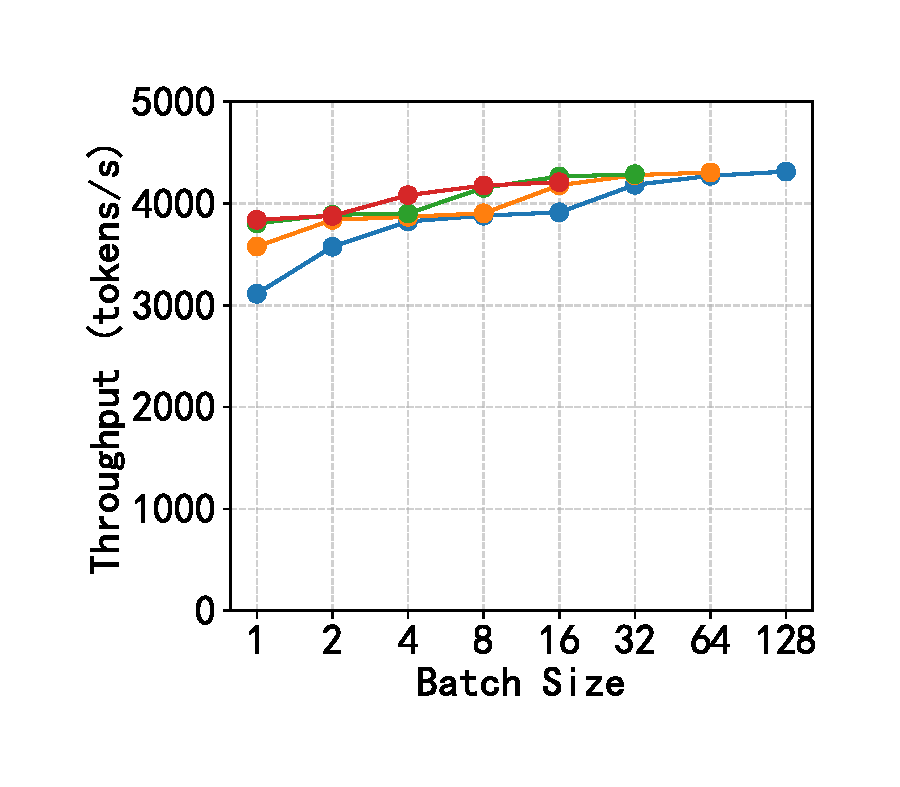
\includegraphics[width=\linewidth]{prefill.pdf}
\end{minipage}
}
    \hfill
    \subfloat[Decode phase.\label{fig:moti1-decode}]{%
\begin{minipage}{0.48\linewidth}
\centering
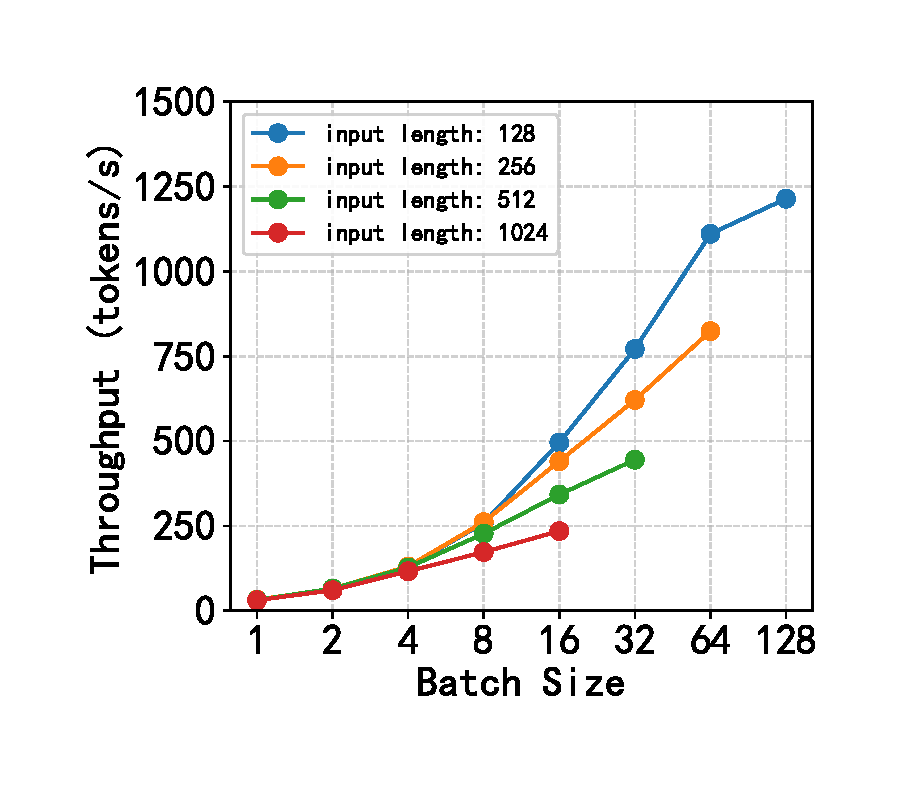
\includegraphics[width=\linewidth]{decode.pdf}
\end{minipage}
}
    \caption{Throughput of the two inference phases under different batch sizes and sequence lengths (LLaMA-3.1 8B on a single RTX 3090 GPU). Prefill saturates once prompt processing reaches the device's compute limit, whereas decode continues to scale with batch size until memory bandwidth becomes the bottleneck.}
    \label{fig:moti1}
\end{figure}

\subsection{Generative LLM Inference}\label{2.1}

Decoder-only LLMs \cite{b1,b2,b3,transformer} generate text autoregressively. From a systems perspective, inference naturally decomposes into two sequential phases: prefill and decode.

\textbf{Prefill.}
In the prefill phase, the model processes the entire input prompt, computes hidden states for all input tokens, constructs the initial KV cache, and produces the first output token. Since all prompt tokens are processed together across Transformer layers, prefill exposes substantial matrix-computation parallelism and is predominantly compute-intensive. Its dominant cost is strongly correlated with input length, which makes prefill cost largely predictable before execution.

\textbf{Decode.}
In the decode phase, the model generates one token per iteration. Although each step introduces only one new token, attention must read the accumulated KV cache from all prior tokens. As a result, decode performs relatively little new computation per step but incurs substantial memory traffic, especially under concurrency. Decode is therefore typically more sensitive to memory bandwidth and token-level queuing delay than raw compute throughput.

These differences imply that TTFT and TPOT are governed by different resource bottlenecks. TTFT is dominated by prefill execution and prefill-side queueing delay, whereas TPOT is dominated by decode-side iteration latency and KV-cache pressure.

Figure~\ref{fig:moti1} illustrates this asymmetry empirically. As prompt length grows, prefill throughput eventually plateaus, indicating that the device has entered a compute-saturated regime. In contrast, decode throughput continues to improve as batch size increases until memory bandwidth becomes the limiting factor. This distinction is central to our design: prefill and decode are not merely two steps of the same pipeline, but two workload classes with different bottlenecks and different scheduling signals.

\subsection{Existing Optimizations and Their Limits}\label{2.2}

Modern LLM serving systems rely on batching, memory management, and phase separation to improve performance. These techniques are essential, but none of them fully address the scheduling mismatch exposed by heterogeneous phase-disaggregated workloads.

\textbf{Batching and continuous scheduling.}
Batching amortizes model execution cost across requests and is therefore a primary mechanism for improving throughput. However, naive static batching is ineffective for LLMs because input and output lengths vary widely, causing severe straggler effects. Systems such as Orca \cite{orca}, vLLM \cite{vllm}, and TensorRT-LLM \cite{tensorrt} therefore adopt \emph{continuous batching}, allowing requests to join and leave a running batch dynamically. While this substantially improves utilization, it still does not resolve the fundamental mismatch between prefill and decode when both are scheduled within the same domain.

\textbf{KV-cache memory management.}
The KV cache grows with sequence length and can occupy a large fraction of GPU memory, directly limiting concurrency. vLLM \cite{vllm} addresses this issue with PagedAttention, which allocates KV state incrementally in fixed-size blocks rather than reserving large contiguous buffers upfront. This design improves memory efficiency and batching capacity. Nevertheless, better KV allocation alone does not determine which requests should be served first, nor does it address the phase-specific nature of prefill and decode scheduling.

\textbf{Phase-disaggregated architectures.}
Recent systems such as Splitwise \cite{b5}, D\'ej\`aVu \cite{b6}, and DistServe \cite{distserve} separate prefill and decode onto different instances. This removes direct phase interference and enables phase-specific resource provisioning. However, once the two phases are separated, each phase still faces its own internal scheduling bottleneck. Prefill remains vulnerable to batching inefficiency caused by highly skewed prompt lengths, while decode remains vulnerable to straggler effects caused by unknown generation lengths.

The limitation of existing approaches is therefore not the absence of batching, memory optimization, or disaggregation per se. Rather, it is the absence of a \emph{phase-specialized scheduling framework} that explicitly matches the scheduling policy to the information structure of each phase.

\subsection{Problems and Opportunities}\label{2.3}

We now empirically characterize the inefficiencies that persist even after phase disaggregation. Our findings show that the two phases exhibit different failure modes and should be treated as different scheduling problems.

\begin{figure}[t]
    \centering
    \subfloat[Prompt length distribution in ShareGPT.\label{fig:share_prefill_tongji}]{%
\begin{minipage}{0.48\linewidth}
\centering
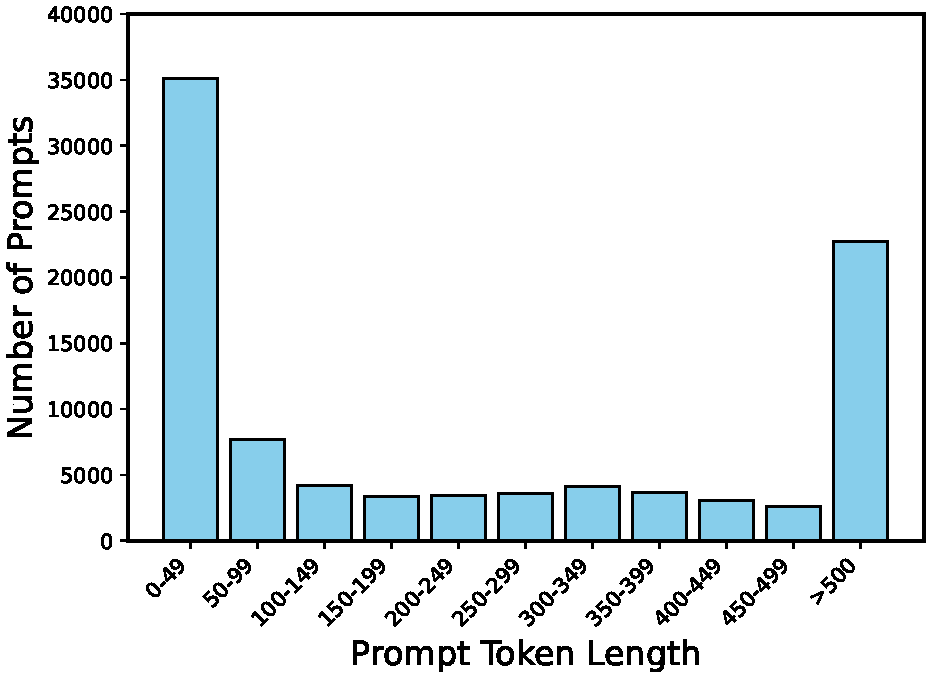
\includegraphics[width=\linewidth]{share_prefill_tongji.pdf}
\end{minipage}
}
    \hfill
    \subfloat[Prefill latency under mixed prompt lengths.\label{fig:problem_prefill}]{%
\begin{minipage}{0.48\linewidth}
\centering
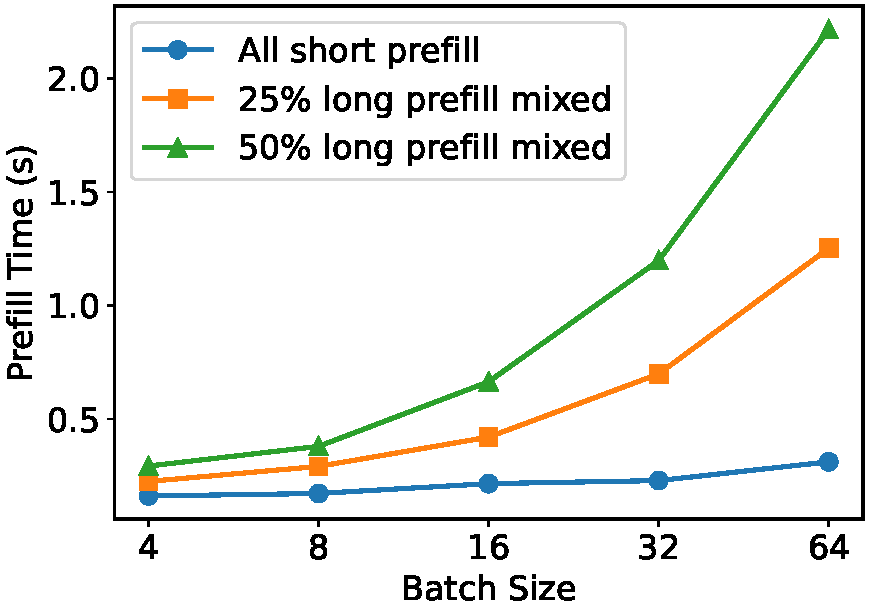
\includegraphics[width=\linewidth]{problem_prefill.pdf}
\end{minipage}
}
    \caption{Empirical evidence of prefill-side heterogeneity. Real workloads exhibit highly skewed prompt lengths, and mixing short and long prompts in the same batch significantly inflates prefill latency.}
    \label{fig:prefill-inter}
\end{figure}

\noindent\textbf{Observation 1: Prefill is a scheduling problem with known but highly skewed job sizes.}
Prompt lengths in real workloads vary substantially, and this variation directly determines prefill cost. Figure~\ref{fig:share_prefill_tongji} shows the prompt-length distribution of ShareGPT, which is highly skewed: short prompts are common, but long prompts remain frequent enough to create substantial heterogeneity. This workload shape implies that prefill naturally corresponds to a scheduling setting in which job sizes are largely known but highly imbalanced.

We further measure the impact of mixing short and long prompts in the same prefill batch. Figure~\ref{fig:problem_prefill} shows that when only a fraction of long prompts is introduced into an otherwise short-prompt batch, overall prefill latency increases sharply. The reason is that prefill execution time is dominated by the longest sequence in the batch. Shorter requests are therefore forced to wait behind longer ones, inflating TTFT and reducing effective compute utilization. Importantly, this inefficiency is not eliminated by continuous batching or by phase disaggregation itself, because it is rooted in the mismatch between skewed prompt costs and batch-level execution semantics.

\begin{figure}[t]
    \centering
    \subfloat[Decode latency under mixed output lengths.\label{fig:decode-time}]{%
\begin{minipage}{0.48\linewidth}
\centering
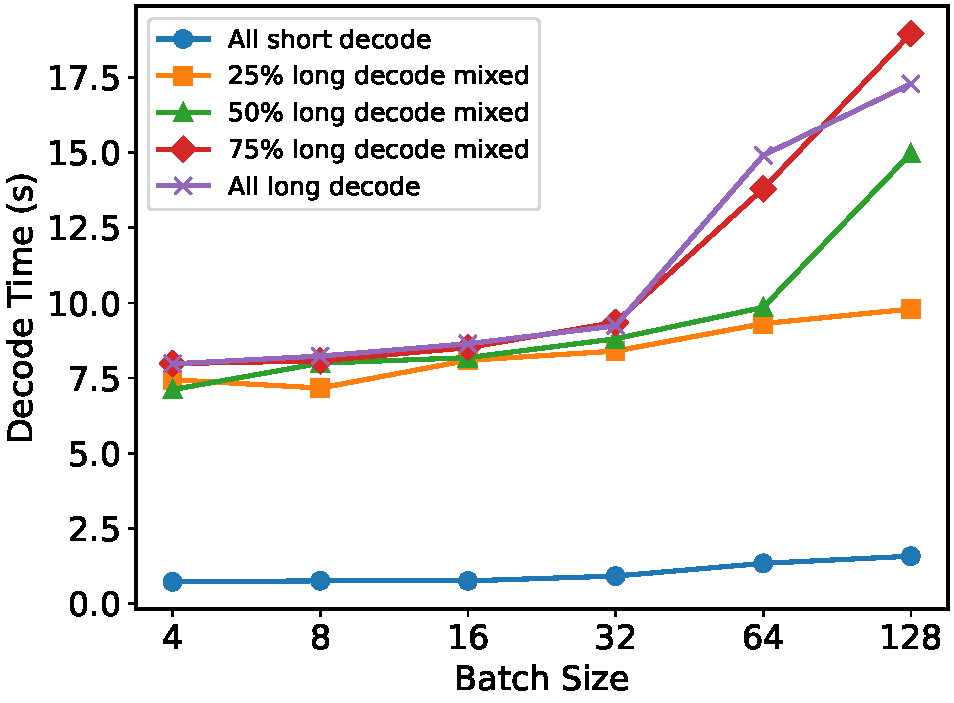
\includegraphics[width=\linewidth]{decode-time.pdf}
\end{minipage}
}
    \hfill
    \subfloat[Decode throughput under mixed output lengths.\label{fig:decode_throughput}]{%
\begin{minipage}{0.48\linewidth}
\centering
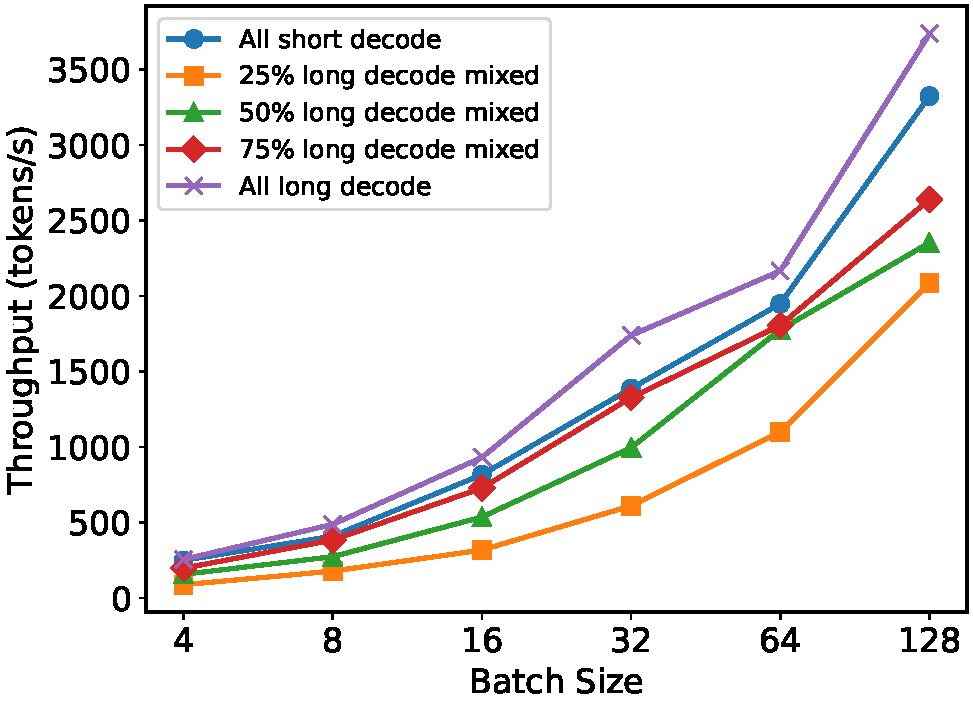
\includegraphics[width=\linewidth]{decode_throughput.pdf}
\end{minipage}
}
    \caption{Empirical evidence of decode-side heterogeneity. Long generations remain in the system for many more iterations, causing straggler effects that increase latency and reduce throughput for short requests.}
    \label{fig:decode-inter}
\end{figure}

\noindent\textbf{Observation 2: Decode is a scheduling problem with unknown and dynamically revealed job sizes.}
Decode exhibits a fundamentally different structure. While the cost of each individual iteration is relatively stable, the total number of iterations required by a request is unknown a priori and varies significantly across requests. Figure~\ref{fig:decode-inter} shows that mixing short and long generations in the same decode workload significantly increases latency and reduces throughput. Long-running requests remain active for many more iterations, thereby occupying decode slots and delaying the completion of short requests.

This behavior is a classic straggler phenomenon. Unlike prefill, however, it cannot be effectively addressed by simple size-based grouping or static batching, because the total generation length is not known in advance. Instead, the scheduler must make decisions online based on attained service and evolving request state.

\noindent\textbf{Design implication.}
These observations reveal that the bottlenecks of phase-disaggregated serving are not uniform. Prefill corresponds to a scheduling regime with known job sizes and highly skewed cost distribution, suggesting size-aware batching and bounded-wait prioritization. Decode corresponds to an iterative scheduling regime with unknown job sizes, suggesting service-aware scheduling with explicit fairness and state management. Therefore, an efficient PD serving system should not apply a single generic policy to both phases. Instead, it should explicitly align each phase with the scheduling signals and control mechanisms appropriate to its workload structure.

This insight motivates the design of PhaseServe. Rather than treating phase disaggregation as the end of optimization, PhaseServe treats it as the beginning of a new scheduling regime: once prefill and decode are separated, each phase should be scheduled according to its own information structure, bottleneck, and latency objective.


















\section{PhaseServe Design}\label{design}

\subsection{Overview}

PhaseServe is a phase-disaggregated LLM serving system that targets \emph{SLO-constrained goodput}: it seeks to maximize the sustainable request rate while satisfying both TTFT and TPOT targets for the vast majority of requests. The design is motivated by a simple but important observation: after prefill and decode are disaggregated, the main bottlenecks no longer come only from direct phase interference, but also from \emph{intra-phase heterogeneity} and \emph{cross-phase imbalance}. Prefill requests have known but highly heterogeneous execution costs before execution, whereas decode requests reveal their total service demand only incrementally as tokens are generated. As a result, the two phases require fundamentally different local scheduling policies, and the system as a whole requires explicit cross-phase control.

\begin{equation}
\max \ \text{Goodput}
\qquad
\text{s.t.}\quad
\text{TTFT}_{p90}\le \tau_{\text{TTFT}},\;
\text{TPOT}_{p90}\le \tau_{\text{TPOT}}.
\label{eq:global_obj}
\end{equation}

Figure~\ref{fig:overview} shows the architecture of PhaseServe. The system consists of four major components: a \emph{global phase controller}, a pool of \emph{prefill engines}, a pool of \emph{decode engines}, and a \emph{KV-state manager}. Requests first enter the global ingress queue and are routed to a prefill engine. After prefill completes and the initial KV state is materialized, the request is handed off to a decode engine for autoregressive generation. Throughout execution, the KV-state manager tracks the residency and transfer status of request state and exposes this information to both the global controller and local schedulers.

PhaseServe is organized as a hierarchical control system. The \emph{global phase controller} performs coarse-grained decisions on routing, phase balancing, and control-epoch adaptation. Each \emph{prefill engine} performs utility-aware batch construction for known-size jobs, and each \emph{decode engine} performs service-aware iterative scheduling for unknown-size jobs under explicit KV and prefetch budgets. This organization separates long-timescale control from short-timescale dispatch, allowing PhaseServe to react to both dynamic workload composition and iteration-level service variability.

\begin{figure}[t]
\centering
\fbox{
\parbox{0.95\columnwidth}{
\centering
\vspace{0.4em}
\textbf{Placeholder for System Overview Figure}\\[0.4em]
\footnotesize
Recommended drawing: a full pipeline with four blocks:
\textit{Global Phase Controller} $\rightarrow$ \textit{Prefill Engines} $\rightarrow$ \textit{KV-State Manager} $\rightarrow$ \textit{Decode Engines}.\\
Show request arrival at the controller, routing to one prefill engine, prefill completion and KV registration, topology-aware handoff to one decode engine, and iterative token generation.\\
Add feedback arrows from prefill/decode pools back to the controller labeled:
\textit{prefill backlog}, \textit{decode backlog}, \textit{TTFT/TPOT miss rate}, and \textit{KV-transfer pressure}.\\
Inside the controller, annotate four functions:
\textit{load estimation}, \textit{routing}, \textit{phase-balance tuning}, and \textit{policy adaptation}.
\vspace{0.4em}
}
}
\caption{Architecture of PhaseServe. A global phase controller performs routing and closed-loop phase balancing. Prefill engines use utility-aware batch construction for known-size requests. Decode engines use service-aware iterative scheduling under KV-state control. The KV-state manager explicitly tracks residency, prefetch, eviction, and handoff.}
\label{fig:overview}
\end{figure}

\subsection{Global Phase Controller}

The global phase controller is the control plane of PhaseServe. It maintains a lightweight but continuously updated view of system state, including the pending workload of each prefill engine, the active decode backlog of each decode engine, KV-transfer pressure, and observed SLO violations. The controller is invoked on request arrival and at every control epoch.

\subsubsection{Request Characterization and Cost Proxies}

For each request $r$, the controller extracts a compact descriptor
\[
\phi(r)=\langle l_{\text{in}}, \hat{l}_{\text{out}}, s, c \rangle,
\]
where $l_{\text{in}}$ is the input length, $\hat{l}_{\text{out}}$ is an optional coarse output-length class, $s$ denotes the request or SLO class, and $c$ denotes the current context length once the request enters decode.

PhaseServe does not require highly accurate latency prediction. Instead, it relies on robust phase-specific cost proxies that are sufficient for online control. For prefill, the request cost is approximated as
\begin{equation}
\hat{C}_{\text{prefill}}(r)=a_{1}l_{\text{in}} + a_{2}l_{\text{in}}^{2},
\label{eq:prefill_cost}
\end{equation}
which captures the dominant scaling behavior of prompt processing with respect to input length. For decode, the instantaneous cost is approximated as
\begin{equation}
\hat{C}_{\text{decode}}(r)=b_{1}c + b_{2}m_{\text{kv}}(r),
\label{eq:decode_cost}
\end{equation}
where $m_{\text{kv}}(r)$ denotes the KV-cache footprint of request $r$. This proxy reflects both context growth and decode-side memory pressure.

\subsubsection{Phase-Specific Load Estimation}

Using these proxies, the controller maintains phase-specific load estimates. For a prefill engine $e_p$, the estimated load is
\begin{equation}
\hat{L}_{p}(e_p)=\sum_{r \in Q_{p}(e_p)} \hat{C}_{\text{prefill}}(r),
\end{equation}
where $Q_{p}(e_p)$ includes both queued and currently executing prefill requests. For a decode engine $e_d$, the estimated load is
\begin{equation}
\hat{L}_{d}(e_d)=\sum_{r \in A(e_d)} \hat{C}_{\text{decode}}(r),
\end{equation}
where $A(e_d)$ is the active decode set.

This separation is important. Prefill pressure is dominated by known prompt-processing cost, whereas decode pressure is dominated by iterative context growth, KV footprint, and activation cost. A single aggregated load signal would obscure this asymmetry and lead to unstable routing.

\subsubsection{Routing and Topology-Aware Handoff}

Upon arrival, a request is routed to the prefill engine minimizing
\begin{equation}
\text{Score}_{p}(e_p,r)=w_{1}\hat{L}_{p}(e_p)+w_{2}\hat{Q}_{p}(e_p)+w_{3}\text{SLOPenalty}(e_p,r),
\label{eq:prefill_route}
\end{equation}
where $\hat{Q}_{p}(e_p)$ denotes queueing pressure and $\text{SLOPenalty}(e_p,r)$ estimates the TTFT risk for request $r$ on engine $e_p$.

After prefill completes, the request is forwarded to the decode engine minimizing
\begin{equation}
\text{Score}_{d}(e_d,r)=u_{1}\hat{L}_{d}(e_d)+u_{2}T_{\text{kv}}(e_p,e_d,r)+u_{3}\text{NetCost}(e_p,e_d),
\label{eq:decode_route}
\end{equation}
where $T_{\text{kv}}(e_p,e_d,r)$ estimates the KV-state handoff cost from prefill engine $e_p$ to decode engine $e_d$, and $\text{NetCost}(e_p,e_d)$ captures topology-dependent communication cost. This formulation makes routing explicitly state-aware: decode placement is treated as a joint scheduling-and-handoff decision rather than a pure queue-balancing problem.

\subsubsection{Closed-Loop Phase Balancing}

Phase disaggregation removes direct prefill--decode interference, but also introduces a producer--consumer relation between the two phases. Under realistic workloads, prefill may over-produce requests relative to decode capacity, or decode may be underutilized because prefill has become the bottleneck. To address this issue, the controller operates in repeated control epochs. At the end of each epoch, it collects four signals:
\begin{itemize}
    \item prefill backlog growth,
    \item decode backlog growth,
    \item TTFT/TPOT SLO miss rate,
    \item KV-transfer saturation.
\end{itemize}

Based on these signals, the controller updates three classes of parameters:
\begin{itemize}
    \item \textbf{prefill aggressiveness}, including the waiting-window size and target prefill workload;
    \item \textbf{decode aggressiveness}, including queue quanta, starvation threshold, and admission conservativeness;
    \item \textbf{cross-phase balance}, including routing weights and the effective prefill/decode capacity ratio.
\end{itemize}

In effect, the controller acts as a slow-timescale optimizer layered above the local schedulers. Local engines react to instantaneous request heterogeneity, while the controller corrects structural imbalance across epochs. This separation keeps the control plane lightweight while still allowing the system to adapt to non-stationary workloads.

\subsection{Prefill Engine}

The prefill engine executes prompt processing and first-token generation. Since the dominant cost of a prefill request is known before execution, PhaseServe models prefill scheduling as an online problem with known but highly heterogeneous job sizes. The engine consists of two tightly coupled mechanisms: \emph{windowed candidate selection} and \emph{utility-aware batch construction}.

\subsubsection{Windowed Candidate Selection}

Instead of greedily batching every newly arrived request, the prefill engine collects requests within a bounded waiting window $W_p$. Let $\mathcal{R}_p$ denote the set of pending requests in the local queue. At each dispatch round, the engine forms a candidate set
\begin{equation}
\mathcal{C}_{p}=\{r \in \mathcal{R}_{p} \mid \text{wait}(r)\le W_{p}\}\cup\{r_{\text{oldest}}\},
\label{eq:candidate_prefill}
\end{equation}
where $r_{\text{oldest}}$ is always included to prevent starvation. This design avoids the pathological behavior of purely greedy batching while still bounding request waiting time.

\subsubsection{Utility-Aware Batch Construction}

Within $\mathcal{C}_{p}$, the engine constructs the next prefill batch by maximizing a phase-specific utility:
\begin{equation}
U_{p}(B)=\sum_{r\in B}\omega(r)-\lambda_{1}\text{PadCost}(B)-\lambda_{2}\text{LoadGap}(B)-\lambda_{3}\text{MemRisk}(B),
\label{eq:prefill_utility}
\end{equation}
where $\omega(r)$ is a request weight that increases with waiting age and decreases with estimated cost, $\text{PadCost}(B)$ measures inefficiency caused by batching mismatched prompt lengths together, $\text{LoadGap}(B)$ measures the distance between the estimated workload of batch $B$ and the empirically profiled GPU saturation region, and $\text{MemRisk}(B)$ penalizes configurations likely to trigger memory pressure.

Operationally, the engine first ranks candidates using a score that combines estimated cost and age, then greedily builds a memory-feasible batch, and finally performs local refinement to improve workload matching and reduce padding waste. Compared with fixed-count batching, this formulation directly optimizes the latency--utilization tradeoff: short requests are favored in the common case, but memory constraints, batching efficiency, and fairness are all considered simultaneously.

\subsubsection{Bounded-Wait Dispatch}

Pure size-based policies can delay long prompts under sustained load. PhaseServe therefore introduces a dispatch timeout $\tau_p$. If the oldest request in the candidate set has waited longer than $\tau_p$, the engine immediately dispatches the best feasible batch even if the utility is slightly below the preferred saturation target. This yields a bounded-wait implementation of size-aware scheduling: short requests are prioritized when possible, while long requests are protected from indefinite delay.

\noindent\textbf{Algorithm Implementation.}
Algorithm~\ref{alg:prefill-scheduler} implements the prefill-side candidate selection and utility-aware batch construction.

\begin{algorithm}[t]
\small
\caption{Utility-Aware Prefill Scheduling}
\label{alg:prefill-scheduler}
\begin{algorithmic}[1]
\REQUIRE Waiting window $W_p$, candidate set $\mathcal{R}$, memory budget $M_p$, target workload $L_m$, dispatch timeout $\tau_p$
\ENSURE Next prefill batch $B^\star$

\STATE $B^\star \leftarrow \emptyset$
\STATE $\mathcal{C} \leftarrow \{r \mid r \in \mathcal{R},\; \text{wait}(r)\le W_p \text{ or } r \text{ is oldest}\}$

\FORALL{$r \in \mathcal{C}$}
    \STATE estimate $c_r \leftarrow \hat{C}_{\text{prefill}}(r)$
    \STATE estimate $m_r \leftarrow \hat{M}_{\text{prefill}}(r)$
    \STATE compute score $s_r \leftarrow f(c_r,\text{wait}(r),\text{age}(r))$
\ENDFOR

\STATE Sort $\mathcal{C}$ by decreasing $s_r$
\STATE $B \leftarrow \emptyset$

\FORALL{$r \in \mathcal{C}$}
    \IF{$\hat{M}(B \cup \{r\}) \le M_p$}
        \STATE tentatively add $r$ to $B$
        \IF{$U_p(B \cup \{r\}) \ge U_p(B)$}
            \STATE $B \leftarrow B \cup \{r\}$
        \ENDIF
    \ENDIF
\ENDFOR

\STATE Apply local refinement on $B$ to reduce padding waste and improve load matching
\IF{$B = \emptyset$}
    \STATE $B \leftarrow \{\text{oldest request}\}$
\ENDIF

\IF{$\text{oldestWait}(\mathcal{C}) \ge \tau_p$}
    \STATE $B^\star \leftarrow B$
\ELSIF{$\hat{L}(B)\ge L_m$}
    \STATE $B^\star \leftarrow B$
\ENDIF

\STATE \textbf{return} $B^\star$
\end{algorithmic}
\end{algorithm}

\begin{figure}[t]
\centering
\fbox{
\parbox{0.95\columnwidth}{
\centering
\vspace{0.4em}
\textbf{Placeholder for Prefill Scheduling Figure}\\[0.4em]
\footnotesize
Recommended drawing: compare \textit{naive FCFS/fixed-count batching} with \textit{PhaseServe prefill scheduling}.\\
Use a small set of requests with highly different prompt lengths.\\
Top: naive batching places short prompts behind one long prompt and creates a poorly matched batch.\\
Bottom: PhaseServe first forms a candidate window, then builds one or two utility-aware batches whose workload is close to the GPU saturation region.\\
Annotate two benefits: reduced head-of-line blocking and improved workload matching.
\vspace{0.4em}
}
}
\caption{Illustrative example of prefill scheduling under heterogeneous prompt lengths. Compared with naive batching, PhaseServe forms utility-aware batches that better match GPU saturation while reducing head-of-line blocking for short requests.}
\label{fig:prefill}
\end{figure}

\subsection{Decode Engine}

The decode engine performs iterative token generation and directly determines TPOT. Unlike prefill, decode requests do not reveal their total service demand in advance. PhaseServe therefore models decode scheduling as an iterative service-allocation problem with unknown job sizes and explicit memory constraints. The engine combines a \emph{service-aware priority scheduler} with a \emph{KV-state-aware admission mechanism}.

\subsubsection{Service-Aware Priority Model}

Each decode request $r$ maintains a state tuple
\[
\psi(r)=\langle a(r), s(r), q(r), \delta(r) \rangle,
\]
where $a(r)$ is the waiting age, $s(r)$ is the attained service measured in decode iterations, $q(r)$ is the current priority level, and $\delta(r)$ is the TPOT slack relative to the target SLO.

PhaseServe computes a dynamic urgency score
\begin{equation}
P(r)=\beta_{1}\frac{1}{1+s(r)}+\beta_{2}a(r)+\beta_{3}\delta(r)-\beta_{4}\text{PrefetchCost}(r).
\label{eq:decode_priority}
\end{equation}
This score favors lightly served requests, gradually raises the priority of starving requests, accelerates SLO-critical requests, and discounts requests whose immediate activation cost is too high. In this way, PhaseServe approximates attained-service-aware scheduling without requiring knowledge of the remaining output length.

\subsubsection{Hierarchical Queue Organization}

To keep scheduling overhead manageable, the priority model is implemented using a hierarchy of queues derived from MLFQ. Newly admitted decode requests enter the highest-priority queue, and long-running requests are gradually demoted as they accumulate service. However, queue transitions are not determined solely by quantum depletion. They additionally depend on starvation age, SLO slack, and KV activation readiness. As a result, the queue hierarchy acts as a practical approximation to least-attained-service scheduling rather than a blind OS-style time-sharing policy.

Let the decode scheduler maintain $n$ queues $\{Q_1,Q_2,\dots,Q_n\}$, where $Q_1$ has the highest priority. The corresponding quanta satisfy
\begin{equation}
\tau_1 < \tau_2 < \cdots < \tau_n,
\qquad
\tau_{i+1}=2\tau_i.
\label{eq:decode_quanta}
\end{equation}
This exponential structure gives newly arrived or lightly served requests fine-grained responsiveness while amortizing scheduling overhead for long-running requests.

\subsubsection{Memory-Aware Batch Admission}

At each iteration, the decode engine first ranks ready requests by $P(r)$, then admits the next batch subject to memory and prefetch constraints. A request can be admitted only if
\begin{equation}
\texttt{CanAdmit}(r,B)=
\bigl[m_{\text{kv}}(B\cup \{r\}) \le M_d\bigr]
\land
\bigl[p(B\cup \{r\}) \le P_d\bigr]
\land
\bigl[t(B\cup \{r\}) \le T_{\max}\bigr],
\label{eq:can_admit}
\end{equation}
where $M_d$ is the available KV budget, $P_d$ is the prefetch bandwidth budget for the current iteration, and $T_{\max}$ is the maximum runtime token budget supported by the engine. This design ensures that a theoretically urgent request is admitted only if its KV state can be activated without destabilizing the current iteration batch.

\subsubsection{Iteration Execution and Bounded Starvation}

Once a batch is admitted, the engine executes exactly one decode iteration for each selected request. After the iteration, the engine updates attained service, queue level, TPOT slack, and completion status. Finished requests release their KV state immediately. Requests that exceed their local quantum or become non-urgent are demoted. Requests whose starvation timer exceeds a threshold $\alpha$ are promoted. By making decisions only at iteration boundaries, PhaseServe preserves responsiveness while keeping scheduling overhead practical.

\noindent\textbf{Algorithm Implementation.}
Algorithm~\ref{alg:decoding-schedule} implements the decode-side service-aware scheduling and KV-state-aware admission policy.

\begin{algorithm}[t]
\small
\caption{Service-Aware Decode Scheduling}
\label{alg:decoding-schedule}
\begin{algorithmic}[1]
\REQUIRE Incoming decode jobs $J_{\text{in}}$, ready set $\mathcal{R}$, priority queues $Q_1,\dots,Q_n$, KV budget $M_d$, prefetch budget $P_d$, max batch tokens $T_{\max}$, starvation threshold $\alpha$
\ENSURE Next decode batch $B^\star$

\STATE $B^\star \leftarrow \emptyset$

\FORALL{$job \in J_{\text{in}}$}
    \STATE initialize $s(job)\leftarrow 0$, $a(job)\leftarrow 0$
    \STATE mark KV state as \texttt{resident}, \texttt{staged}, \texttt{prefetching}, or \texttt{remote}
    \STATE place $job$ into the highest-priority queue $Q_1$
\ENDFOR

\FORALL{$job \in \mathcal{R}$}
    \STATE update $a(job)$, $s(job)$, and TPOT slack $\delta(job)$
    \STATE compute $P(job)$ according to Eq.~(\ref{eq:decode_priority})
    \STATE adjust queue level or in-queue order according to $P(job)$
    \IF{$a(job)\ge \alpha$}
        \STATE promote $job$ to $Q_1$
    \ENDIF
\ENDFOR

\STATE $\mathcal{C} \leftarrow$ jobs ordered by priority across $Q_1,\dots,Q_n$
\FORALL{$job \in \mathcal{C}$}
    \IF{$\texttt{CanAdmit}(job,B^\star)$}
        \IF{$job$ is not \texttt{resident}}
            \STATE issue prefetch for $job$
        \ENDIF
        \STATE $B^\star \leftarrow B^\star \cup \{job\}$
    \ENDIF
\ENDFOR

\FORALL{$job \in B^\star$}
    \STATE execute one token step for $job$
    \STATE $s(job)\leftarrow s(job)+1$
    \IF{$job$ finishes}
        \STATE release KV state and remove $job$
    \ELSIF{$job$ exhausts its local quantum}
        \STATE demote $job$ to a lower-priority queue
    \ENDIF
\ENDFOR

\STATE evict low-priority non-imminent requests according to the KV eviction policy
\STATE \textbf{return} $B^\star$
\end{algorithmic}
\end{algorithm}

\begin{figure}[t]
\centering
\fbox{
\parbox{0.95\columnwidth}{
\centering
\vspace{0.4em}
\textbf{Placeholder for Decode Scheduling Figure}\\[0.4em]
\footnotesize
Recommended drawing: a two-part figure.\\
Left: requests move across $Q_1,\dots,Q_n$ as attained service increases; starving requests are promoted.\\
Right: KV state transitions \texttt{remote} $\rightarrow$ \texttt{prefetching} $\rightarrow$ \texttt{resident}, followed by possible cold-state eviction back to \texttt{remote}.\\
At the bottom, show that an iteration batch is admitted only for requests whose priority is high enough and whose KV can be activated under memory and prefetch budgets.\\
Annotate three benefits: responsiveness for short jobs, bounded starvation, and controllable memory footprint.
\vspace{0.4em}
}
}
\caption{Illustration of decode scheduling in PhaseServe. Requests are organized by attained service and urgency, admitted subject to KV and prefetch budgets, and updated at iteration boundaries to balance responsiveness, fairness, and throughput.}
\label{fig:decode}
\end{figure}

\subsection{KV-State Manager}

A key design choice in PhaseServe is to elevate KV cache to a first-class managed system resource. The KV-state manager tracks where each request state resides and coordinates prefetch, transfer, and eviction with the local schedulers.

\subsubsection{KV Residency States}

For each active request, the KV-state manager tracks one of four residency states:
\begin{itemize}
    \item \textbf{resident}: the KV state is already in the target GPU memory and can be used immediately;
    \item \textbf{staged}: metadata and address mapping are installed, but the state is not yet fully ready for execution;
    \item \textbf{prefetching}: the state is currently being transferred or restored;
    \item \textbf{remote}: the state is stored in host memory or another device and is not immediately executable.
\end{itemize}

This explicit state machine decouples logical request scheduling from physical state placement. The scheduler reasons about readiness through residency states rather than issuing ad hoc swap operations.

\subsubsection{Proactive Prefetch and Cold-State Eviction}

When a request becomes likely to run in the near future, the decode engine issues a prefetch request before the iteration in which the request is expected to be admitted. Conversely, when memory pressure rises, PhaseServe evicts low-priority, non-imminent requests using a cold-state policy that considers both future urgency and reactivation cost.

Let the KV size of request $r$ be $S_{\text{KV}}(r)$ and the effective transfer bandwidth be $B$. The transfer time is
\begin{equation}
T_{\text{swap}}(r)=\frac{S_{\text{KV}}(r)}{B}.
\label{eq:swap_time}
\end{equation}
PhaseServe attempts to hide this cost by overlapping prefetch with ongoing decode computation whenever possible. The exposed latency is therefore only the portion of transfer time that cannot be hidden behind useful work.

\subsubsection{Prefill-to-Decode State Handoff}

When a prefill engine completes a request, it materializes the initial KV state and registers the handoff with the KV-state manager. The actual handoff to the selected decode engine is then scheduled according to the routing decision and the current transfer budget. Because state movement is explicitly modeled, PhaseServe can trade off locality and balance: a decode engine with slightly higher queue pressure may still be preferred if the state-transfer path is significantly cheaper.

\subsection{Implementation Notes}

PhaseServe is implemented on top of a phase-disaggregated serving runtime. The global controller executes asynchronously with respect to local engine execution and maintains only lightweight summaries instead of per-iteration centralized state. Prefill and decode engines therefore make local decisions independently within the policy envelope set by the controller at each control epoch. This separation keeps the control path lightweight and prevents the controller from becoming a runtime bottleneck.

The design intentionally relies only on low-cost signals such as input length, current context length, queue age, KV footprint, and transfer readiness. This choice avoids the brittleness of exact latency prediction while still exposing enough structure for effective scheduling and control.

\subsection{Discussion}

The design of PhaseServe rests on a simple but important principle: \emph{after prefill and decode are disaggregated, the dominant bottleneck often shifts from inter-phase interference to intra-phase heterogeneity and cross-phase imbalance}. Prefill benefits from known-size, utility-aware batch construction; decode benefits from service-aware iterative scheduling; and the system as a whole benefits from an explicit control plane that reasons about load, state, and topology jointly.

Compared with naive phase-disaggregated serving, PhaseServe makes phase-aware control explicit at three levels. At the \emph{local scheduling level}, it uses different scheduling abstractions for known-size prefill and unknown-size decode. At the \emph{state-management level}, it turns KV cache into an explicitly managed resource that enables concurrency-aware decode scheduling. At the \emph{cross-phase coordination level}, it continuously regulates routing and effective phase balance under non-stationary workloads. Together, these mechanisms allow PhaseServe to simultaneously improve TTFT, TPOT, and overall serving efficiency under realistic heterogeneous workloads.




































\section{Implementation}\label{implementation}
PhaseServe is implemented on top of the open-source DistServe \cite{distserve} framework. Our implementation mainly extends DistServe’s scheduler to support phase-specialized scheduling, including cost-aware request routing, length-aware prefill scheduling with capacity-aware batching, and MLFQ-based decode scheduling with proactive KV-cache management. The system uses NCCL \cite{nccl} for tensor and pipeline parallel communication, and each serving instance is realized as a distributed inference engine built from multiple Ray \cite{ray} actors. Prefill and decode remain fully disaggregated as in DistServe, while a lightweight profiler provides cost estimates that guide scheduling and routing decisions. KV-cache state is managed in block form to support decode-side queue transitions and cache movement with low overhead. Overall, PhaseServe preserves the underlying distributed serving stack of DistServe while adding the mechanisms needed to realize phase-specialized scheduling.

\section{Evaluation}\label{evaluation}
We evaluate PhaseServe to answer the following questions:
\begin{itemize}
    \item Does PhaseServe improve TTFT and TPOT over representative unified and phase-disaggregated baselines?
    \item Do the proposed prefill and decode schedulers contribute complementary benefits?
    \item Under the tested deployment setting, does PhaseServe improve SLO attainment under heterogeneous workloads?
\end{itemize}

We compare PhaseServe against DistServe \cite{distserve}, a representative phase-disaggregated serving system, and vLLM \cite{vllm}, a widely used unified serving engine. We emphasize that our goal is to evaluate the effect of \emph{phase-specialized scheduling} under a fixed deployment setting, rather than to exhaustively benchmark every recent serving runtime.

\subsection{Experimental Setup}
\textit{Testbed}. We deployed PhaseServe in a node consisting of 8 NVIDIA PCIe H20-96 GB GPUs. Each GPU is connected to the other via an NVLink bridge with 900 GB/s bidirectional bandwidth. In addition, the CPU is a 128 vCPU AMD EPYC 9K84 96-core processor with 1200 GB of memory. Our system uses a fully-connected NVLink topology (NV18), where all eight GPUs are directly connected via point-to-point NVLink links. Although the machine spans two NUMA domains, GPU–GPU communication never traverses PCIe or the Root Complex, resulting in a uniform NVLink bandwidth fabric.

\textit{Models}. To evaluate PhaseServe, we employ the OPT\cite{b3} series in our experiments, as they are widely regarded as representative in the research community. The OPT family comprises models of various sizes, ranging from 125 million to 175 billion parameters. We use the OPT-6.7B and OPT-66B models for our evaluation. All model parameters in our experiments are configured with FP16 precision.

\textit{Workloads}. We evaluate the capabilities of PhaseServe using two representative workloads that correspond to common LLM inference scenarios. The dataset statistics used in our experiments are summarized in Table~\ref{tab:datasets}. For chat-oriented inference, we adopt the ShareGPT \cite{sharegpt} dataset, which contains real-world multi-turn conversations collected from ChatGPT users. The dataset features diverse prompt and response lengths, making it well-suited for stress-testing prefill and decode scheduling under highly variable input conditions. For code-generation workloads, we employ the HumanEval \cite{humaneval} benchmark, a widely used dataset for evaluating functional code generation. Compared with dialogue datasets, HumanEval requests typically contain short problem descriptions but require models to generate longer and structurally constrained outputs, providing a complementary workload pattern for testing decode-stage performance and KV-cache management.

\begin{table}[t]
\centering
\caption{Statistics of prompt and output token lengths for the evaluated datasets}
\label{tab:datasets}
\resizebox{\columnwidth}{!}{
\begin{tabular}{lcccccc}
\hline
\textbf{Dataset} 
& \multicolumn{3}{c}{\textbf{Prompt Tokens}} 
& \multicolumn{3}{c}{\textbf{Output Tokens}} \\
\cline{2-4} \cline{5-7}
& \textbf{Avg} & \textbf{Median} & \textbf{P90} 
& \textbf{Avg} & \textbf{Median} & \textbf{P90} \\
\hline
ShareGPT  & 768.2 & 695   & 1556  & 195.9 & 87.0  & 518.0 \\
HumanEval & 131.3 & 117.0 & 225.7 & 53.8  & 45.5  & 106.8 \\
\hline
\end{tabular}
}
\end{table}

\textit{Placement Strategies}. Considering the model, workload characteristics, and SLO attainment targets, DistServe decides the allocation of prefill and decoding instances through simulation. PhaseServe follows a similar approach to define its parallelism strategy, with the instance placement used in our experiments summarized in Table~\ref{tab:placement}.

\begin{table}[t]
\centering
\caption{Placement strategies (TP = tensor parallelism, PP = pipeline parallelism)}
\label{tab:placement}
\begin{tabular}{lcc}
\hline
\textbf{Model} & \textbf{Prefill Placement} & \textbf{Decode Placement} \\
\hline
OPT-6.7B      & TP-2, PP-1 & TP-2, PP-1 \\
OPT-66B      & TP-2, PP-2 & TP-2, PP-2 \\
\hline
\end{tabular}
\end{table}

\textit{Metrics}. We report TTFT and TPOT as the primary latency metrics, and include both median and P90 values to capture typical and tail behavior. We additionally report SLO attainment to measure how often requests satisfy target service thresholds under increasing load.

\subsection{End-to-End Performance}

\begin{figure*}[t]
\centering
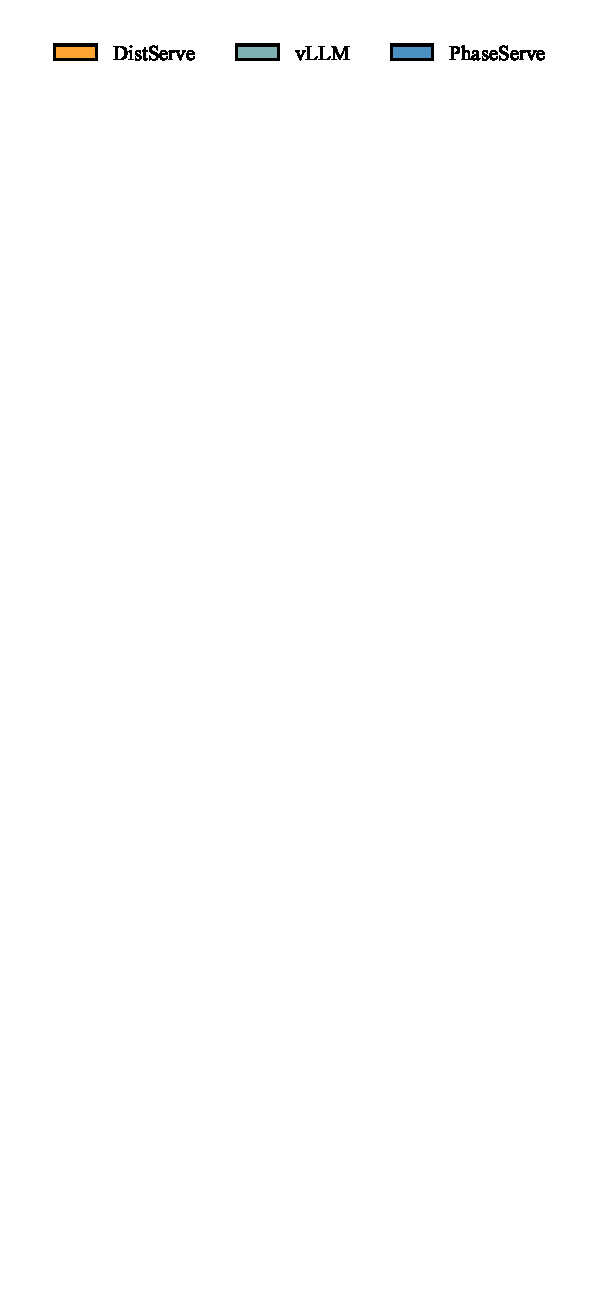
\includegraphics[width=0.3\textwidth]{label.pdf}
\vspace{4pt}

\subfloat[OPT-6.7B on ShareGPT dataset.]{%
    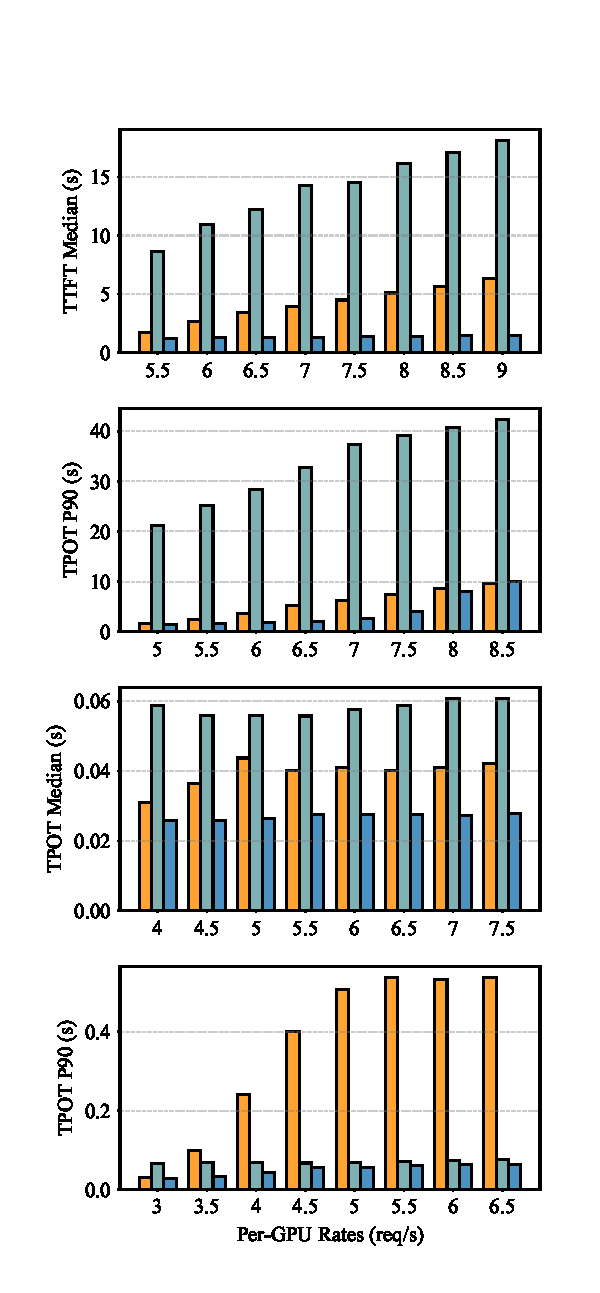
\includegraphics[width=0.24\textwidth]{result1.pdf}%
    \label{fig:opt67b_sharegpt}%
}
\hfill
\subfloat[OPT-6.7B on HumanEval dataset.]{%
    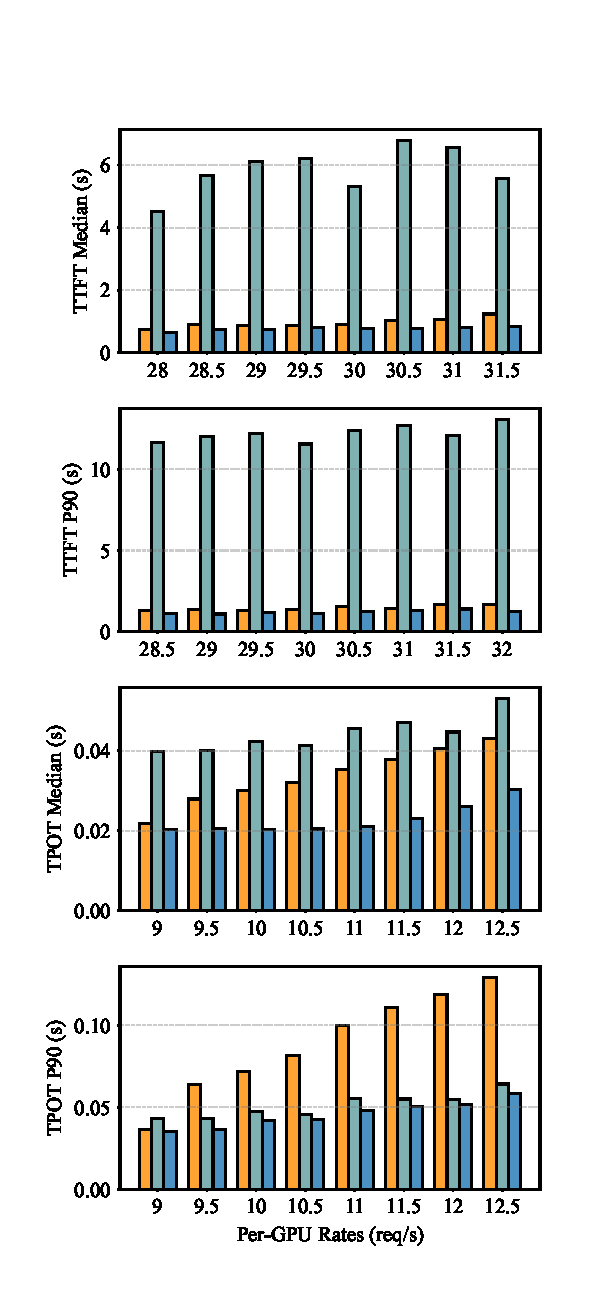
\includegraphics[width=0.24\textwidth]{result2.pdf}%
    \label{fig:opt67b_humaneval}%
}
\hfill
\subfloat[OPT-66B on ShareGPT dataset.]{%
    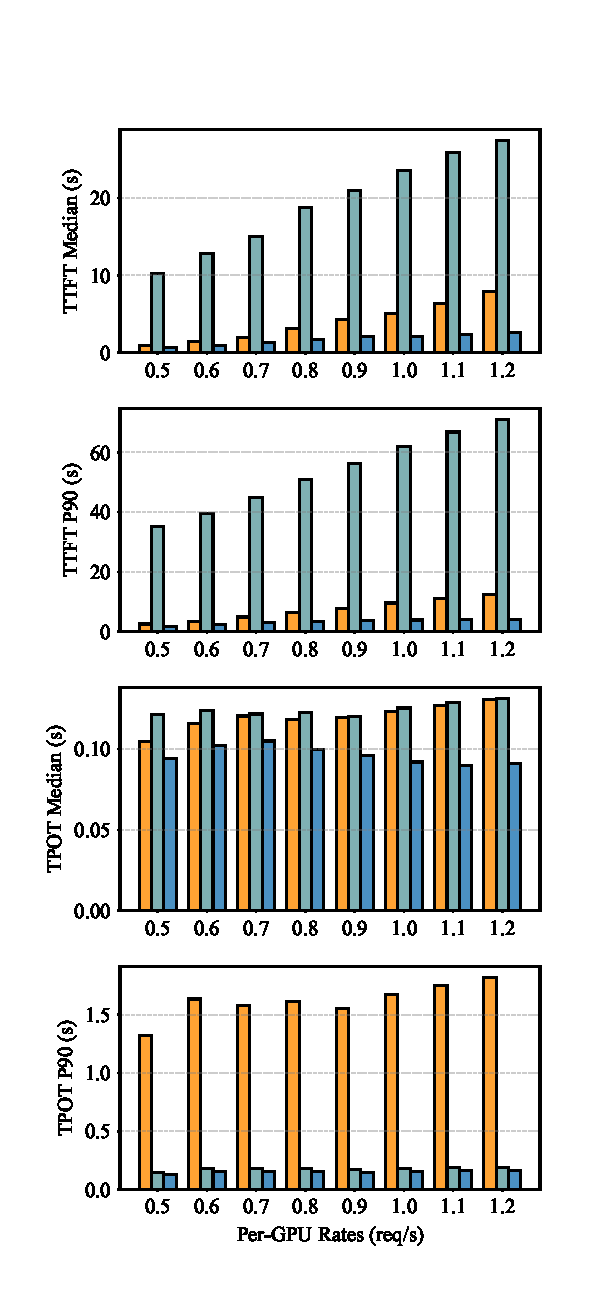
\includegraphics[width=0.24\textwidth]{result3.pdf}%
    \label{fig:opt66b_sharegpt}%
}
\hfill
\subfloat[OPT-66B on HumanEval dataset.]{%
    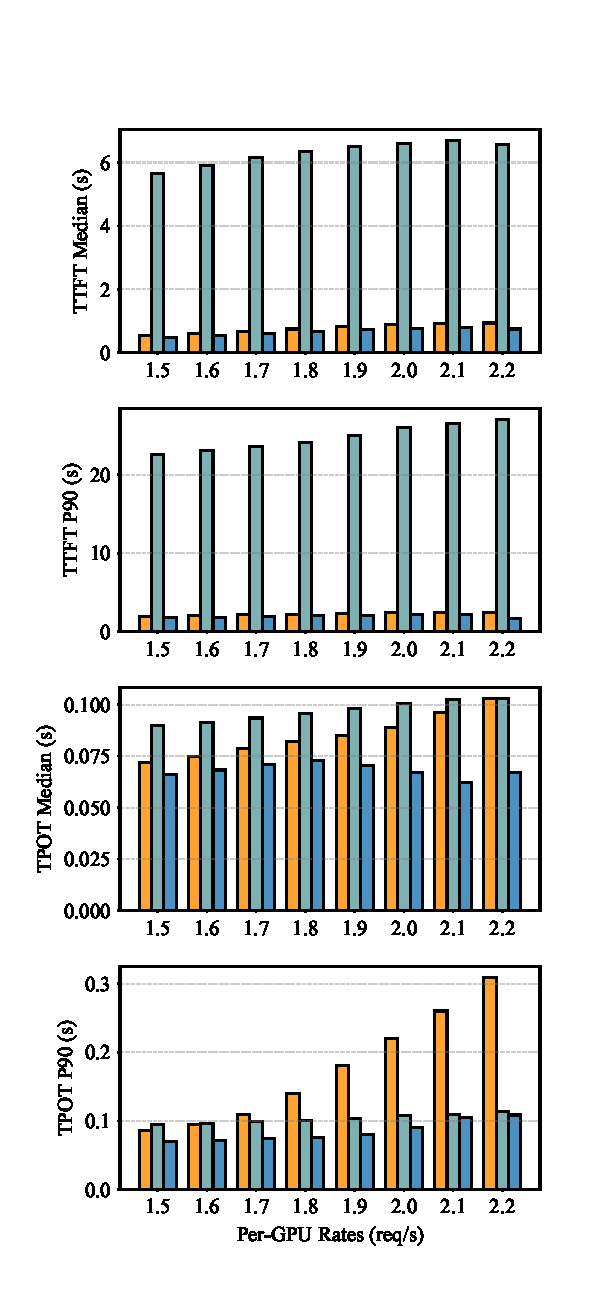
\includegraphics[width=0.245\textwidth]{result4.pdf}%
    \label{fig:opt66b_humaneval}%
}
\caption{End-to-end latency of PhaseServe compared with DistServe and vLLM.}
\label{fig:four-horiz}
\end{figure*}


\textbf{Overall trend.}
Across both workloads and both model scales, PhaseServe consistently reduces TTFT and TPOT relative to the baselines over the tested load ranges. The improvement is especially pronounced in tail latency, indicating that phase-specialized scheduling is particularly beneficial under heterogeneous workloads and increasing contention.

\textbf{ShareGPT.}
Figures~\ref{fig:opt67b_sharegpt} and~\ref{fig:opt66b_sharegpt} show the results on ShareGPT. This workload stresses both prefill scheduling, due to long and highly variable prompt lengths, and decode scheduling, due to diverse response lengths. Under increasing request rate, PhaseServe maintains substantially lower TTFT than both DistServe and vLLM. For example, on OPT-6.7B, when the request rate increases from 5.5 to 9~req/s, PhaseServe keeps median TTFT around 1.2--1.5~s, while DistServe reaches 4--6~s and vLLM exceeds 10~s. This corresponds to approximately 2.5$\times$ speedup over DistServe and up to 5$\times$ over vLLM. Tail TTFT shows a similar trend.

PhaseServe also improves TPOT on ShareGPT. Median TPOT remains around 0.025--0.028~s, corresponding to about 1.4$\times$--1.6$\times$ speedup over DistServe and 2$\times$--2.5$\times$ over vLLM. P90 TPOT remains below 0.06~s over the tested range, whereas DistServe exhibits substantially larger tail latency at high load. These improvements are consistent with the design of PhaseServe: length-aware prefill scheduling reduces queueing and head-of-line blocking for short requests, while attained-service-aware decode scheduling improves responsiveness during iterative generation.

Overall, on the ShareGPT dataset, PhaseServe significantly outperforms both baselines in first-token response and continuous generation, showing that phase-specialized scheduling is effective under long-context and highly variable dialogue workloads.

\textbf{HumanEval.}
Figures~\ref{fig:opt67b_humaneval} and~\ref{fig:opt66b_humaneval} show the results on HumanEval. Compared with ShareGPT, this workload has shorter prompts and relatively lighter prefill pressure, but still exposes decode-side variability. PhaseServe continues to outperform both baselines on TTFT and TPOT. On OPT-6.7B, when the request rate is 28--31.5~req/s, median TTFT remains at 0.65--0.85~s, compared with 0.9--1.2~s for DistServe and 4--6~s for vLLM. This corresponds to about 1.5$\times$ speedup over DistServe and up to 9$\times$ over vLLM. P90 TTFT follows the same pattern, remaining at 1.1--1.4~s while vLLM exceeds 12~s.

For TPOT, PhaseServe maintains median TPOT latency around 0.02--0.03~s, lower than DistServe (0.03--0.04~s) and vLLM (0.04--0.05~s), corresponding to about 1.5$\times$ speedup over DistServe and about 2$\times$ over vLLM. P90 TPOT remains around 0.06~s across the tested range.

The HumanEval results suggest that the benefit of PhaseServe is not limited to long-prompt dialogue workloads. Even when prefill heterogeneity is less severe, decode-side scheduling still provides measurable latency gains.

\textbf{Interpretation.}
Taken together, these results support the main claim of this paper: once prefill and decode are disaggregated, the remaining latency bottlenecks are largely intra-phase rather than inter-phase. PhaseServe improves performance by matching scheduling policy to phase characteristics: known-size scheduling for prefill and unknown-size scheduling for decode. The effect is most visible in tail latency, where heterogeneous workloads would otherwise amplify queueing and straggler effects.

\subsection{SLO Attainment}

The SLO attainment results are shown in Figure~\ref{fig:SLO}, and the thresholds are summarized in Table~\ref{tab:SLO}. Across the tested rates, PhaseServe consistently achieves higher SLO attainment than DistServe. On ShareGPT, at a per-GPU request rate of 4.5~req/s, PhaseServe improves TTFT and TPOT SLO satisfaction by 1.21$\times$ and 1.94$\times$, respectively.

\begin{figure}[t]
    \centering
    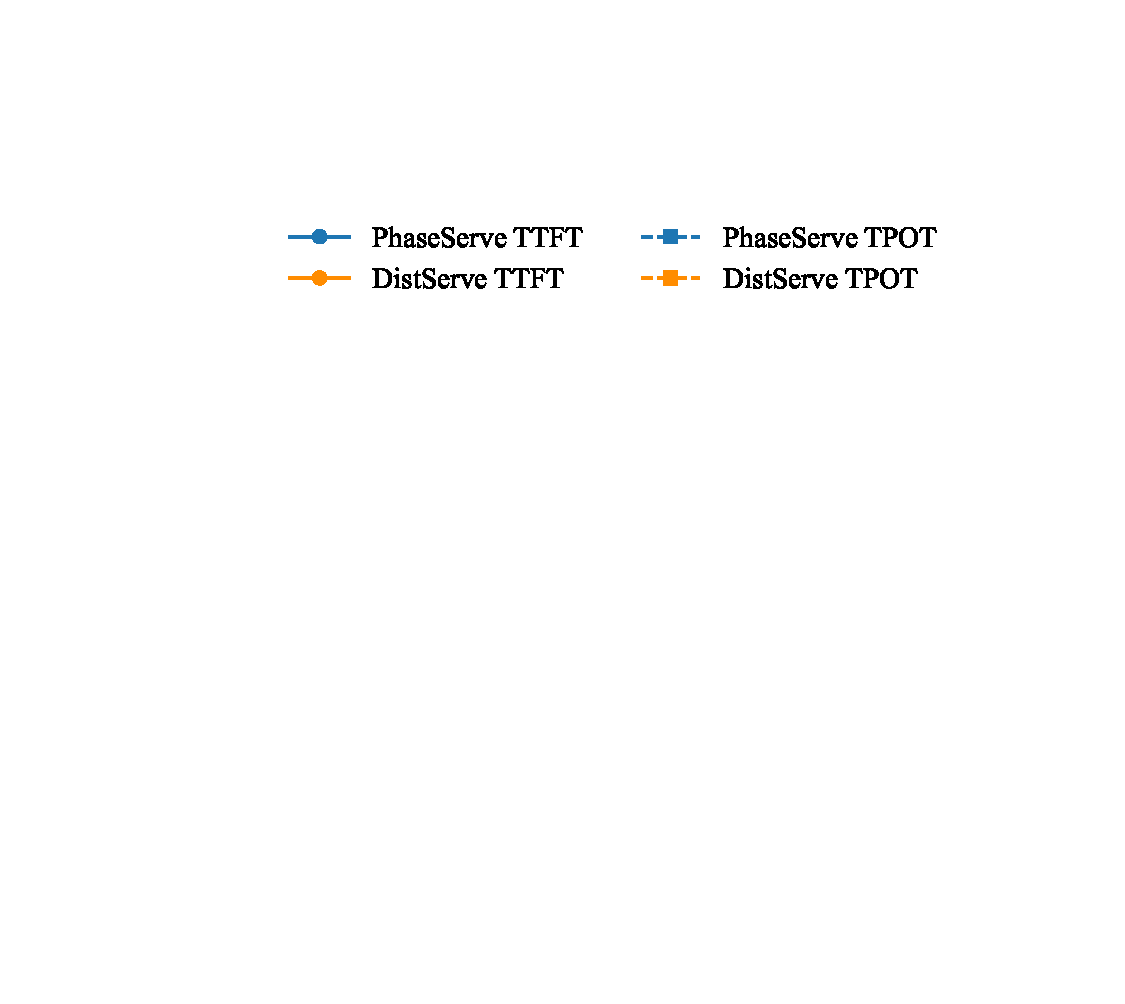
\includegraphics[width=0.6\linewidth]{label-SLO.pdf}
    \vspace{0.1em}

    \subfloat[SLO on ShareGPT dataset.]{
        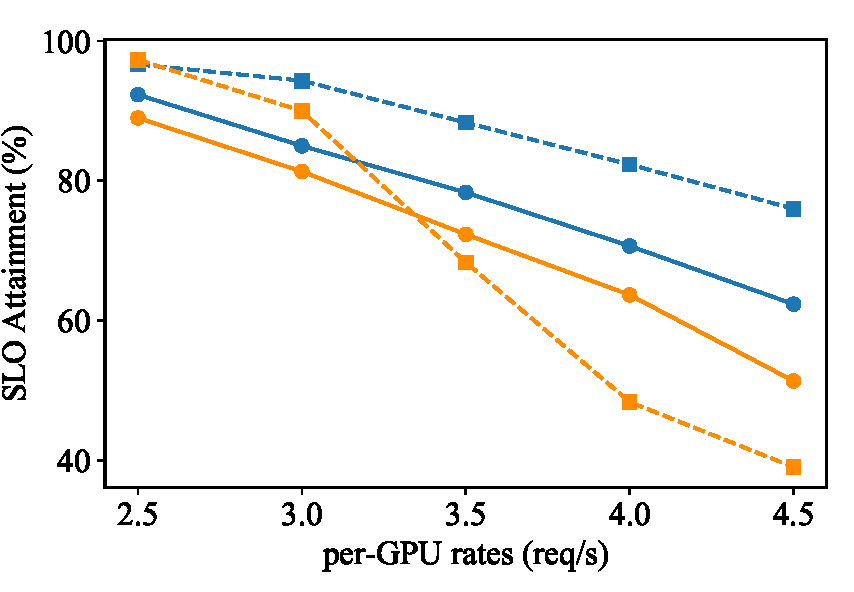
\includegraphics[width=0.48\linewidth]{67b-share-SLO.pdf}
        \label{fig:67b-share-SLO}
    }
    \hfill
    \subfloat[SLO on HumanEval dataset.]{
        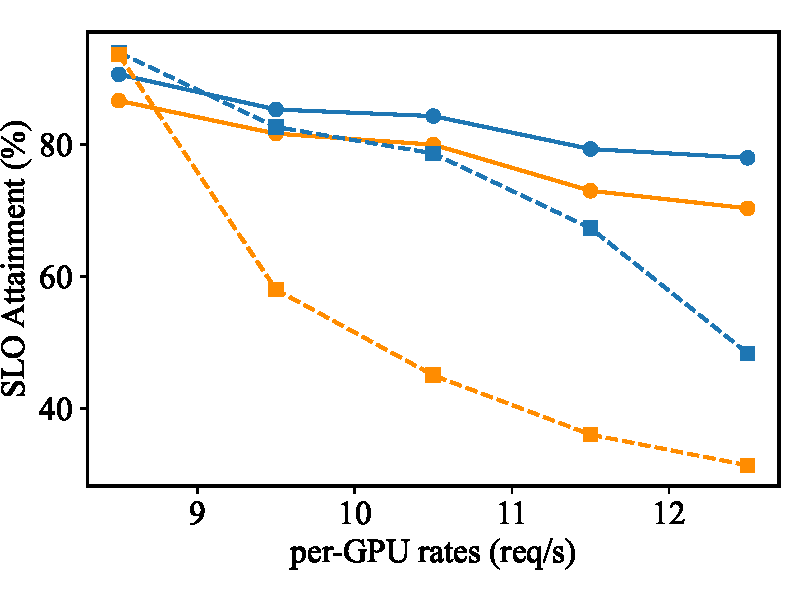
\includegraphics[width=0.46\linewidth]{67b-humaneval-SLO.pdf}
        \label{fig:67b-humaneval-SLO}
    }

    \caption{SLO attainment rates on OPT-6.7B.}
    \label{fig:SLO}
\end{figure}

\begin{table}[t]
\centering
\caption{Absolute SLO thresholds used in the evaluation.}
\label{tab:SLO}
\begin{tabular}{lccc}
\hline
\textbf{Model} & \textbf{Dataset} & \textbf{TTFT (s)} & \textbf{TPOT (s)} \\
\hline
OPT-6.7B & ShareGPT  & 0.4 & 0.03 \\
OPT-6.7B & HumanEval & 0.1 & 0.03 \\
\hline
\end{tabular}
\end{table}

These results complement the latency curves by showing that the gains of PhaseServe are not limited to average-case behavior. Instead, they translate into a higher fraction of requests meeting service targets under load. This is particularly important for production settings, where predictable latency often matters more than peak throughput alone.

At the same time, the absolute SLO values also indicate that the tested configuration eventually becomes overloaded as request rate increases. We therefore interpret SLO attainment primarily as a comparative measure across systems under the same deployment setting, rather than as a claim that all workloads satisfy strict production targets at the highest tested load.

\subsection{Ablation Studies}



In this section, we study the individual effects of the prefill and decode schedulers in PhaseServe. We construct two variants: \textsc{PhaseServe-no-prefill-scheduler}, which replaces the prefill-side length-aware scheduling and capacity-aware batching with a DistServe-style FCFS policy and fixed batch size; and \textsc{PhaseServe-no-decode-scheduler}, which replaces the MLFQ-based decode scheduler with a DistServe-style FCFS policy in the decoding phase. We evaluate these variants on the OPT-6.7B model.

\begin{figure}[htbp]
\centering
\subfloat[TTFT P90 latency]{%
    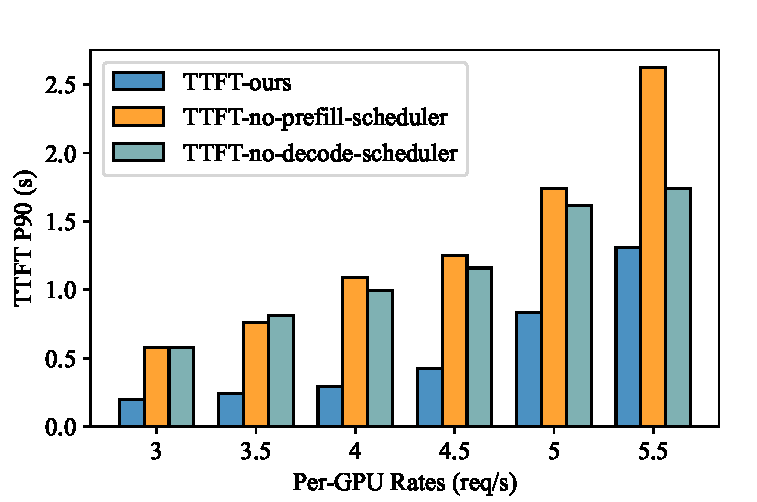
\includegraphics[width=0.49\columnwidth]{ablation1.pdf}%
}
\hfill
\subfloat[TPOT P90 latency]{%
    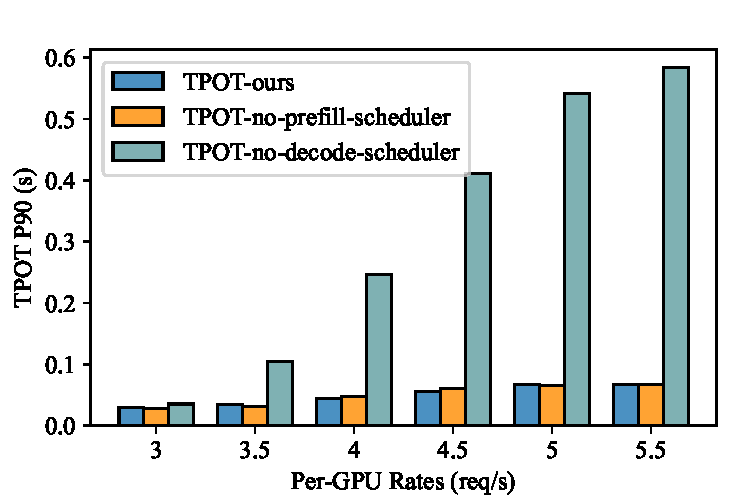
\includegraphics[width=0.49\columnwidth]{ablation2.pdf}%
}
\caption{Ablation Studies}
\label{fig:ablation}
\end{figure}

As shown in Figure~\ref{fig:ablation}, disabling the prefill scheduler results in a noticeable increase in TTFT, particularly at higher request rates. This indicates that the prefill-side design of PhaseServe---namely length-aware request ordering and capacity-aware batch construction---is effective in reducing head-of-line blocking and queueing delay under heterogeneous prompt lengths. In contrast, disabling the decode scheduler primarily degrades TPOT, leading to higher token-level latency under load. This result is consistent with the role of the MLFQ-based scheduler in prioritizing lightly served requests and improving responsiveness during iterative decoding.

PhaseServe with both schedulers enabled consistently achieves the best overall latency profile across the tested per-GPU rates. These results suggest that the two schedulers provide complementary benefits: the prefill scheduler mainly improves request-entry latency, while the decode scheduler mainly improves generation-stage responsiveness.

Overall, the evaluation consistently shows that PhaseServe improves TTFT, TPOT, and SLO attainment under the tested deployment setting. These results support our central claim that, after prefill and decode are disaggregated, intra-phase scheduling remains a dominant source of latency, and that phase-specialized scheduling is effective in reducing this bottleneck.



\section{Related Work}\label{relatedwork}
\textbf{Inference Serving Optimization.} Recent research on LLM inference serving spans general-purpose systems such as Triton \cite{triton}, as well as LLM-specific solutions like Orca \cite{orca}, vLLM \cite{vllm}, and SARATHI \cite{sarathi}. These systems improve throughput and hardware utilization through techniques such as iterative or continuous batching, paged-attention for KV-cache management, and chunked-prefill with piggybacked decoding. However, most prior work colocates prefill and decoding on the same instance, which can lead to interference, pipeline bubbles, and underutilized resources. To address this, disaggregated prefill-decode architectures have been proposed by DistServe \cite{distserve}, Splitwise \cite{b5}, DéjàVu \cite{b6}, separating stages across instances to enable independent scheduling and better resource utilization. PhaseServe builds on this idea but focuses on practical scheduling and batch management within each phase—length-aware scheduling and capacity-aware batch construction in prefill, and MLFQ with KV-cache management in decode.

\textbf{Model Parallelism.} LLMs with hundreds of billions of parameters require parallel execution across multiple GPUs. Prior work \cite{alpaserve, megatron, alpa, pope, hetegen, exegpt, helix} has explored various strategies for model partitioning and scheduling. Pope \cite{pope} propose analytical models for selecting multi-dimensional partitioning strategies tailored to TPU slices. HeteGen \cite{hetegen} introduces heterogeneous parallelism across CPUs and GPUs, leveraging asynchronous overlap to mitigate I/O bottlenecks. ExeGPT \cite{exegpt} optimizes batch size and tensor parallelism degree based on input/output distributions to maximize throughput under latency constraints. Helix \cite{helix} formulates model partitioning across heterogeneous GPUs and network links as a max-flow problem, capturing both compute and communication heterogeneity. PhaseServe can integrate these model-parallelism techniques into its distributed inference engine, enabling flexible and efficient scaling of LLM workloads.

\textbf{Kernel-Level Optimizations.} Efficient attention computation is critical for LLM inference. Techniques such as FlashAttention \cite{flashattention} and FlashAttention-2 \cite{flashattention2} reduce memory access overhead between GPU high-bandwidth memory and on-chip SRAM, improving compute efficiency for long-context sequences. Concurrent approaches like POD-Attention \cite{pod} optimize GPU utilization for hybrid batches, enabling concurrent execution of prefill and decode tasks. Other works explore sparse attention to reduce memory footprint, though they may compromise generation accuracy. PhaseServe is orthogonal to these kernel-level optimizations: our work focuses on scheduling and resource management at the serving-system level, and can be naturally combined with optimized attention kernels to further improve throughput and efficiency.

\section{Conclusion and Future Work}
\label{conclusion}
In this work, we presented PhaseServe, a phase-disaggregated LLM serving system built around the observation that prefill and decoding exhibit fundamentally different scheduling characteristics. Prefill requests have known but highly heterogeneous execution costs, whereas decode requests reveal their total cost only incrementally during generation. Motivated by this asymmetry, PhaseServe applies phase-specialized scheduling to the two stages: length-aware scheduling with capacity-aware batch construction for prefill, and MLFQ-based attained-service-aware scheduling with proactive KV-cache management for decoding.

Our results show that, under the tested deployment setting, this design consistently improves both TTFT and TPOT over representative unified and phase-disaggregated baselines. These findings suggest that, even after prefill and decode are separated, intra-phase scheduling remains a major source of latency and resource inefficiency, and that aligning scheduling policy with phase characteristics is an effective way to address this bottleneck.

There are several promising directions for future work. First, our current study focuses on a single-node NVLink-connected environment; extending PhaseServe to multi-node deployments would enable a deeper understanding of how phase-specialized scheduling interacts with cross-node KV transfer and network heterogeneity. Second, PhaseServe currently assumes a fixed prefill/decode deployment configuration. Incorporating dynamic resource reallocation and heterogeneous hardware support would further improve adaptability under changing workload conditions.

More broadly, we believe that treating prefill and decoding as distinct scheduling regimes provides a useful perspective for future LLM serving systems, especially as deployment environments and workload diversity continue to grow.

%%
%% The acknowledgments section is defined using the "acks" environment
%% (and NOT an unnumbered section). This ensures the proper
%% identification of the section in the article metadata, and the
%% consistent spelling of the heading.

\section*{Acknowledgment}
This work was supported by the open research fund of Pengcheng Laboratory under Grant 2025KF1A0020, and the Joint Funds of the National Natural Science Foundation of China under Grant U22A2036.

\bibliographystyle{IEEEtran}
\bibliography{refs}

\begin{IEEEbiography}[{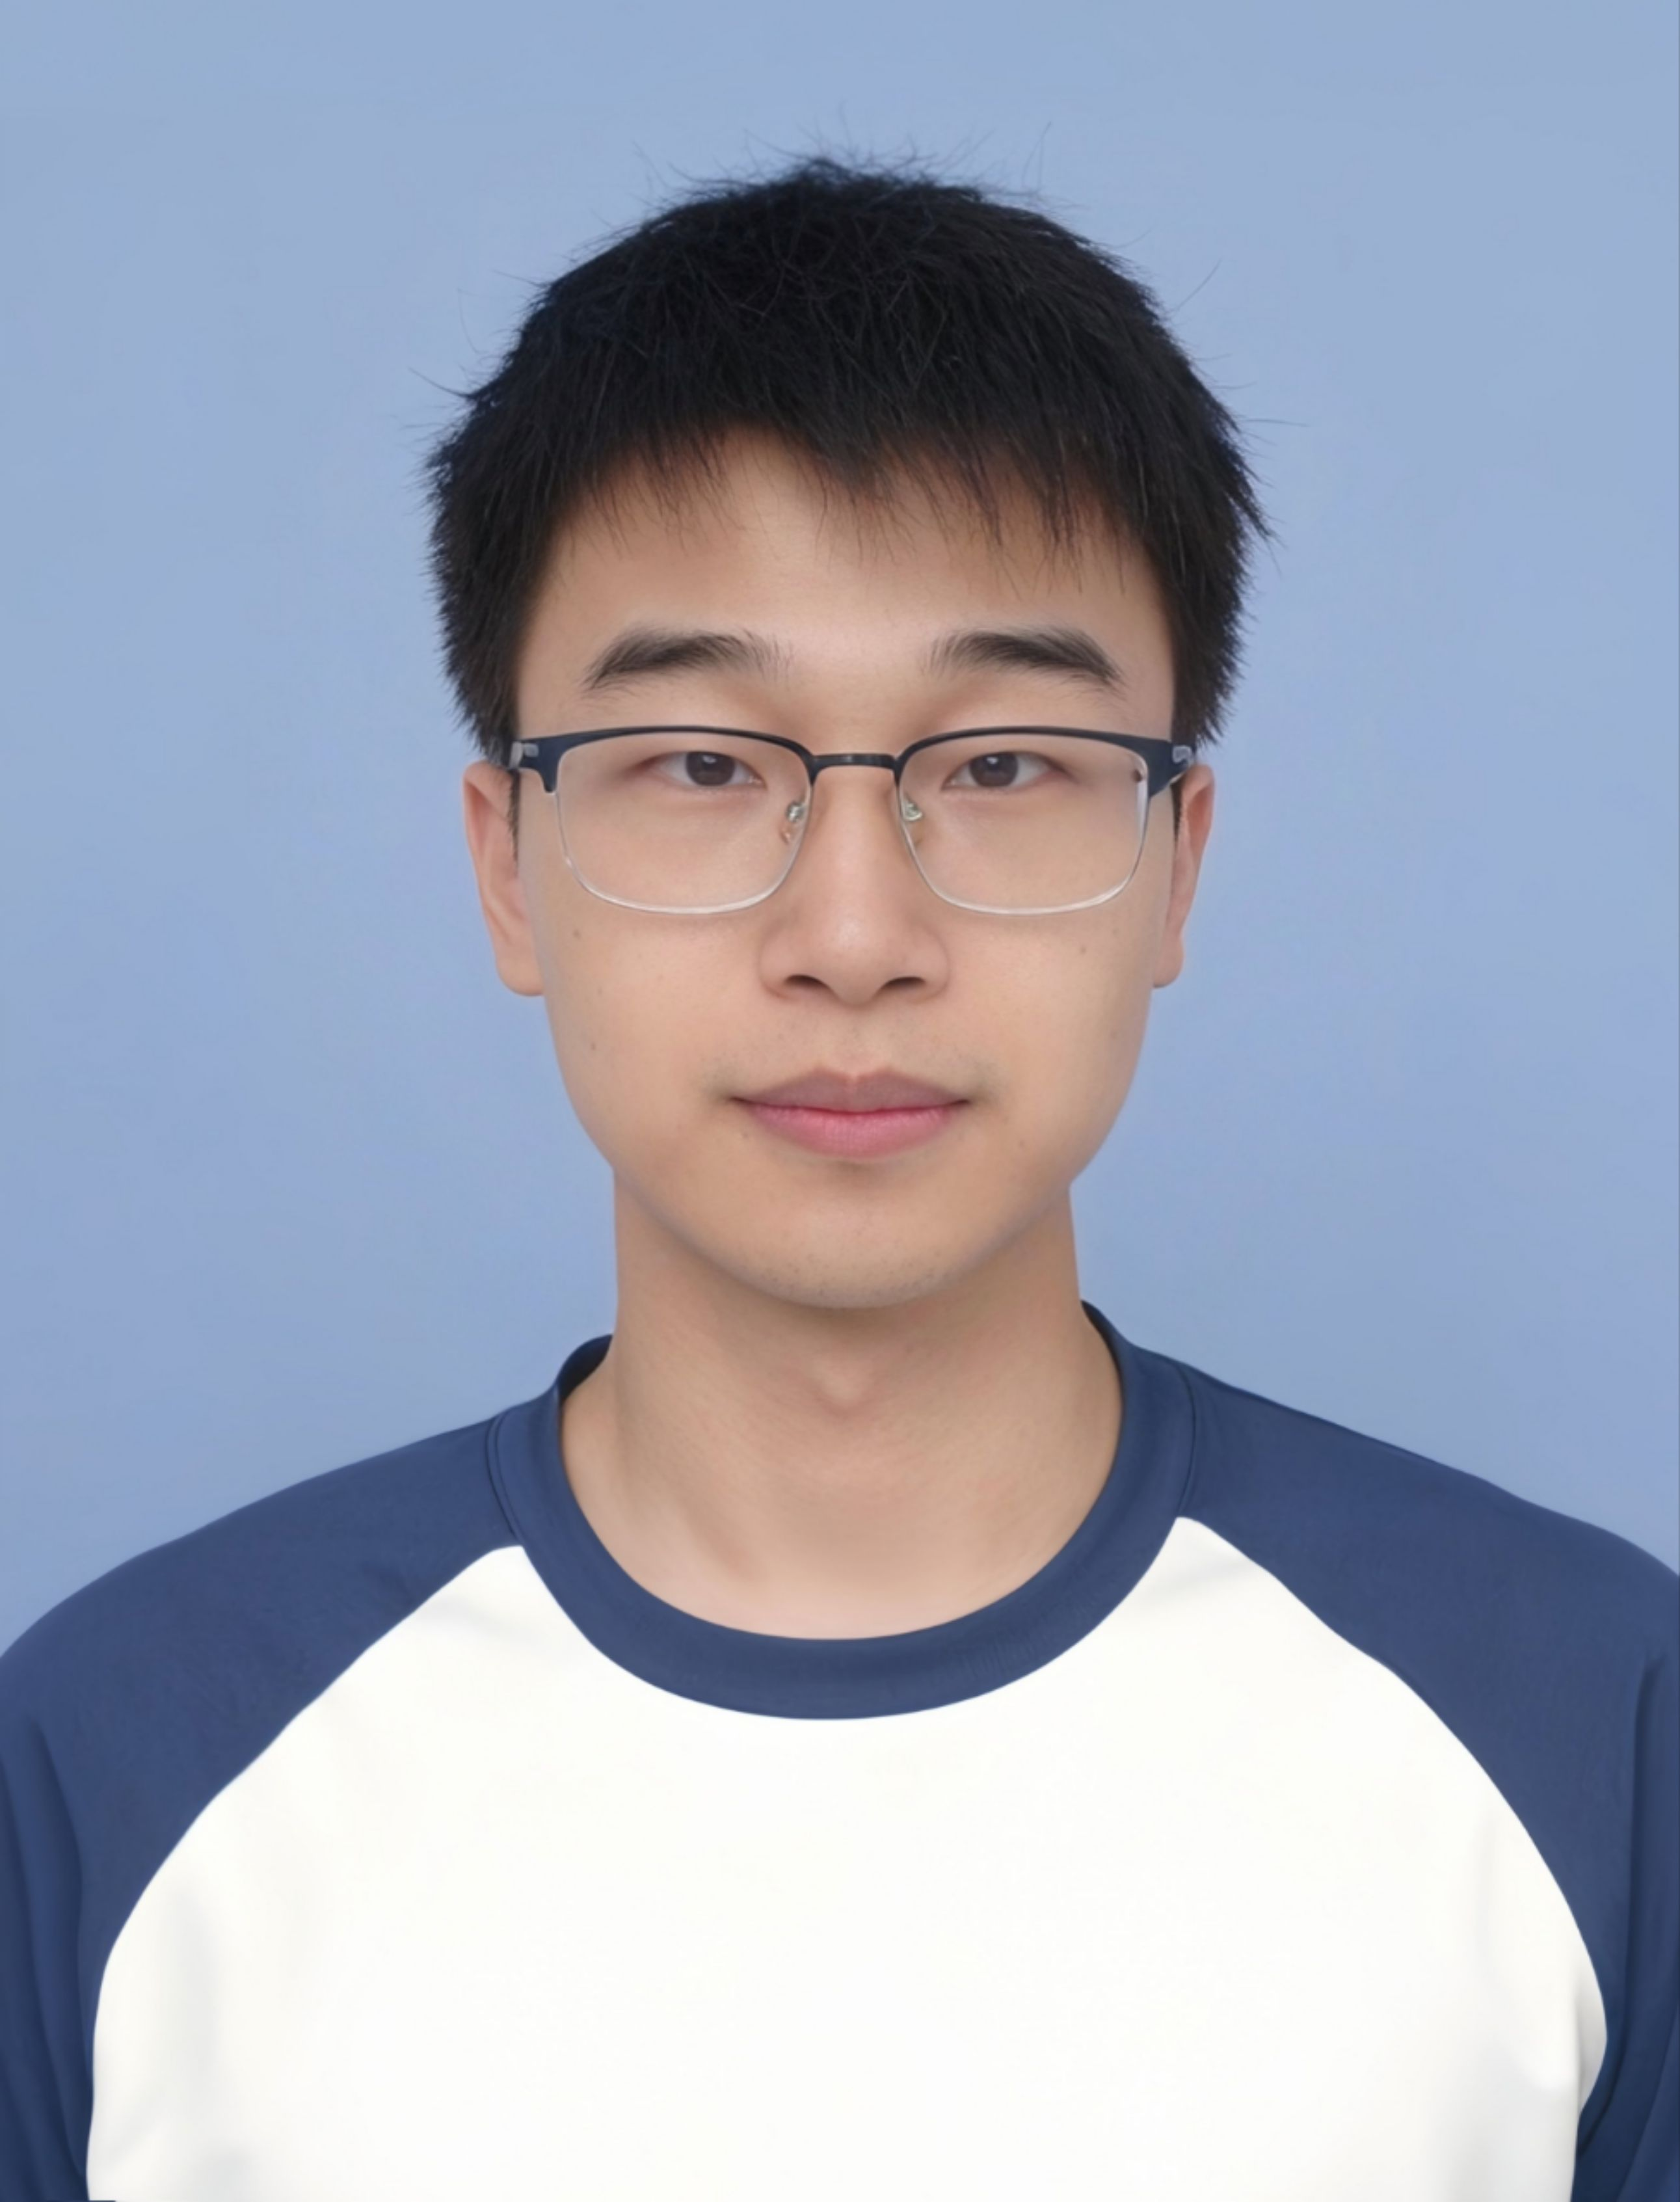
\includegraphics[width=0.8in,height=1.15in,clip,keepaspectratio]{bio/Figure_Dai_Jie.jpg}}]{Jie Dai} obtained his Bachelor's degree in Information Security from Harbin Institute of Technology, China, in 2024. He is currently pursuing his Master's degree at the School of Computer Science and Technology at Harbin Institute of Technology. His research interest lies in large language model inference optimization.
\end{IEEEbiography}
\vspace{-1.2cm}
\begin{IEEEbiography}[{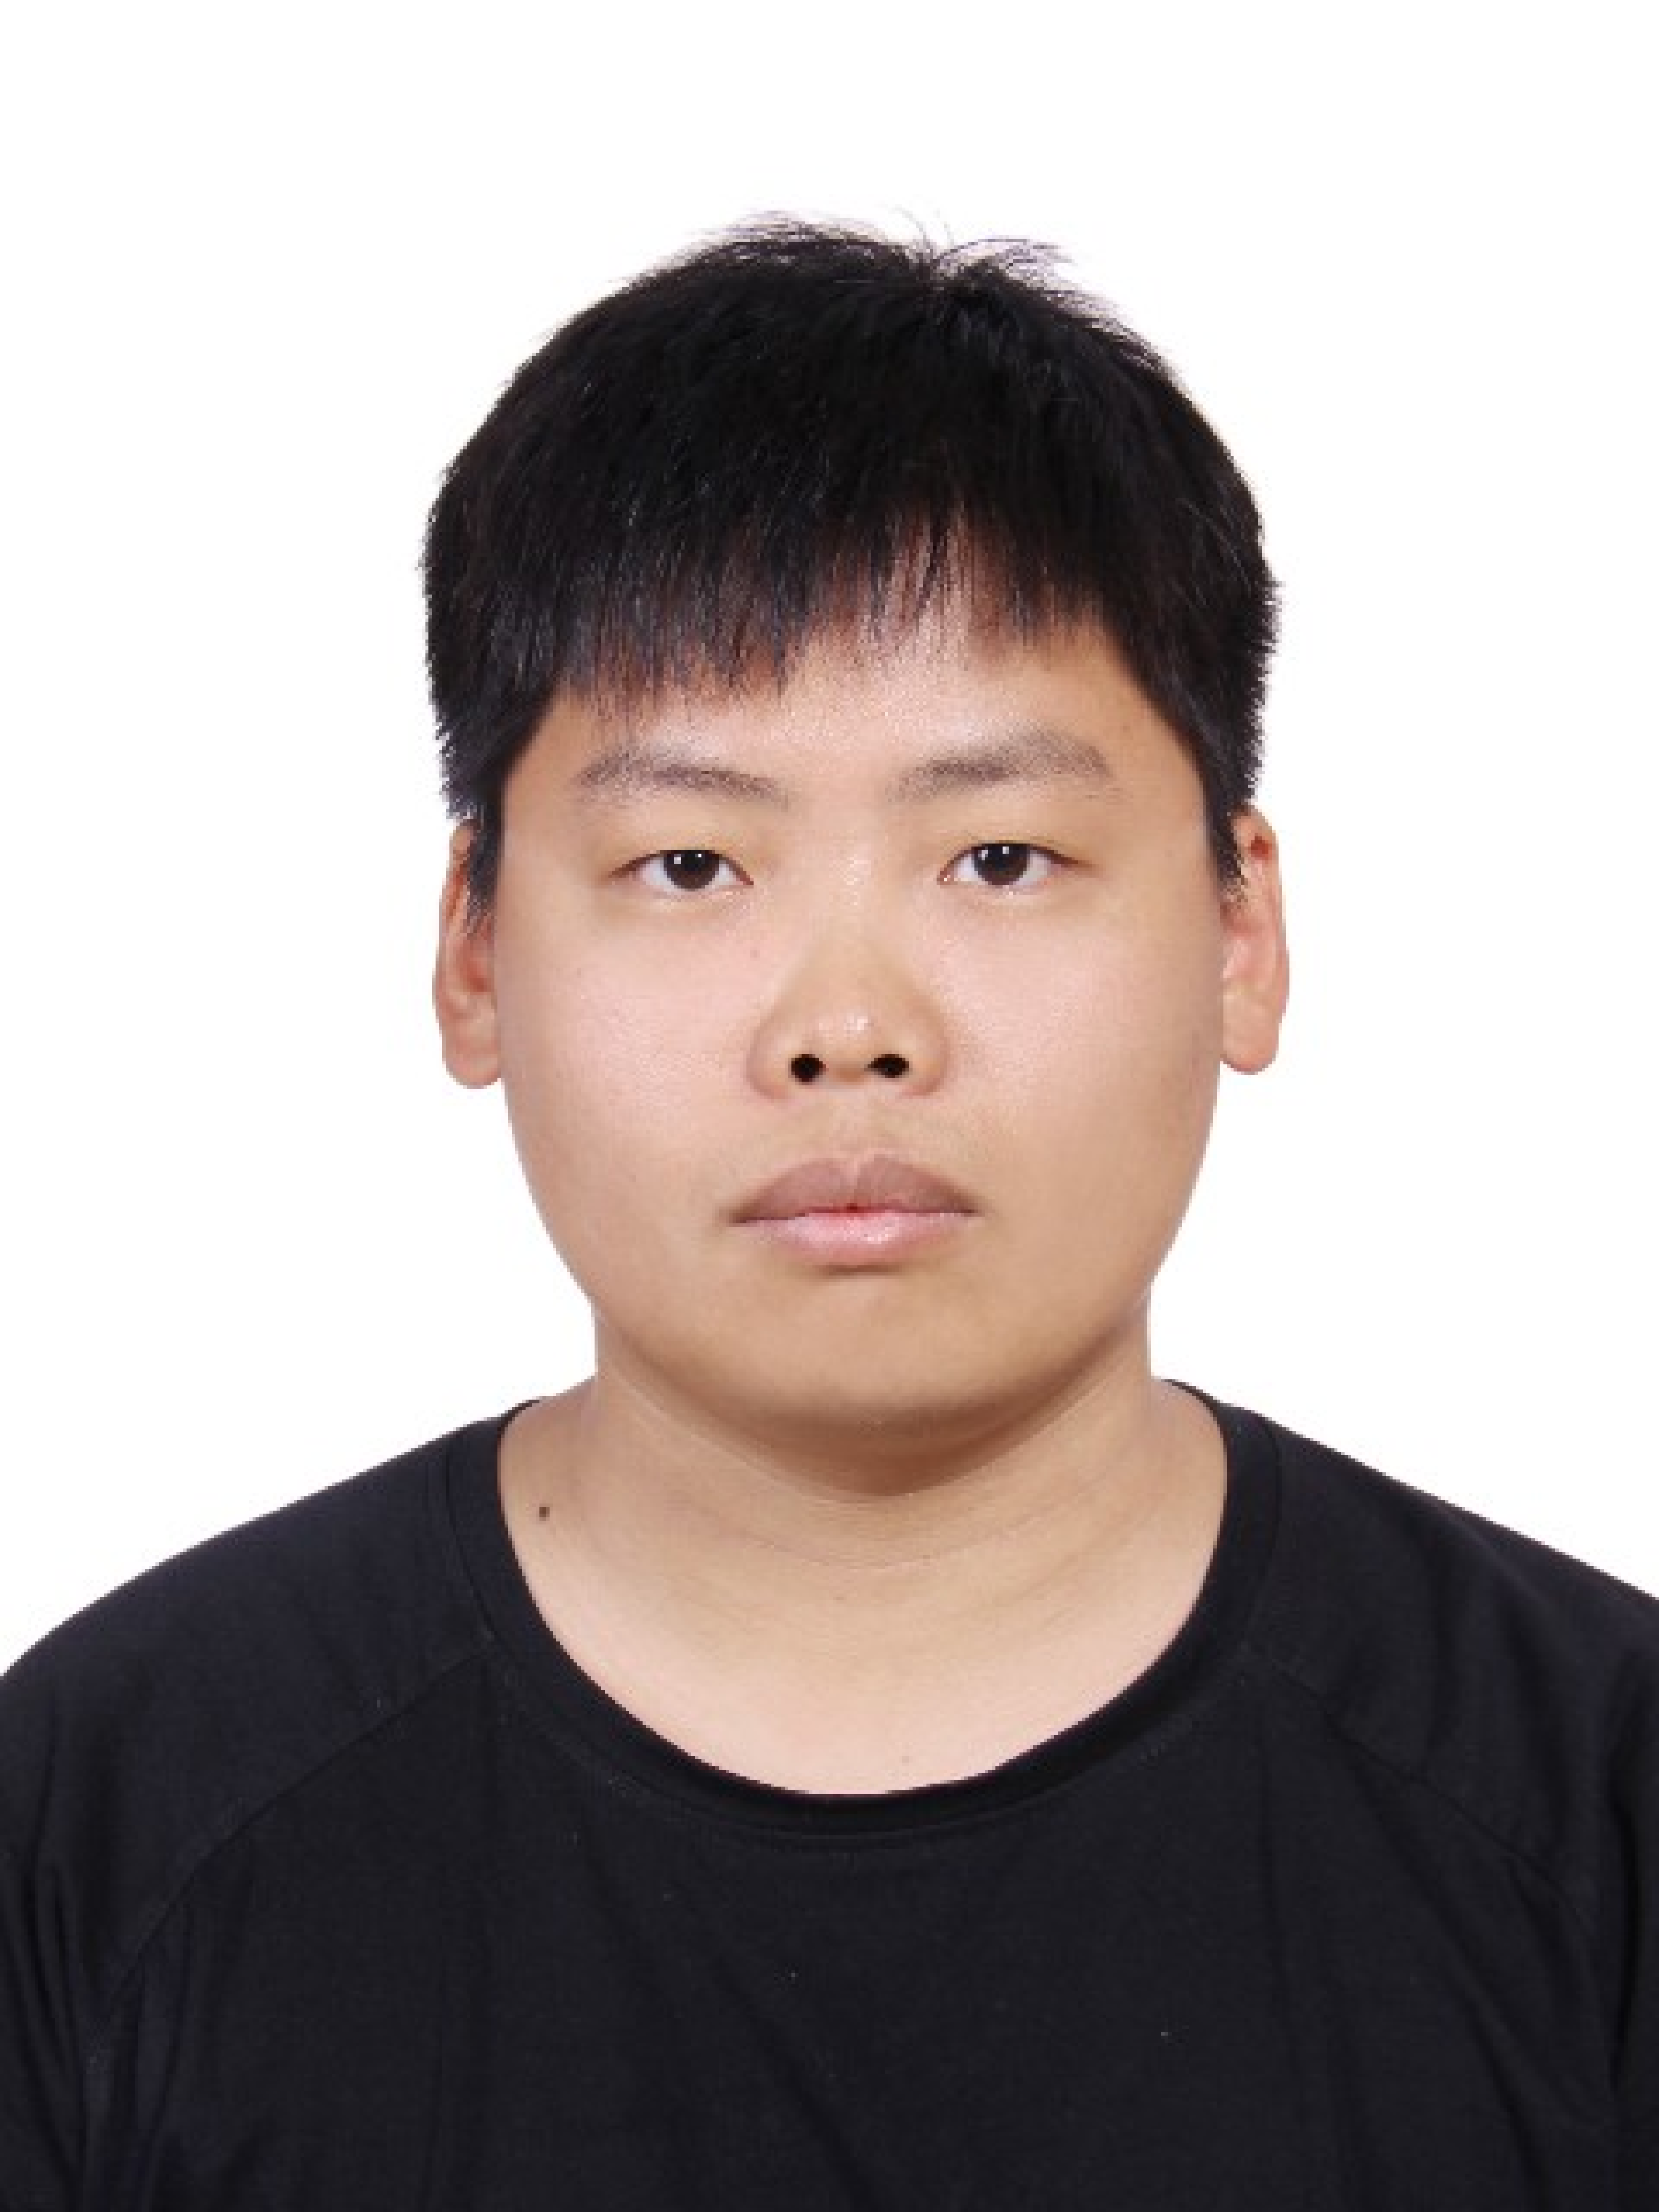
\includegraphics[width=0.8in,height=1.15in,clip,keepaspectratio]{bio/Figure_Hao_Meng.png}}]{Meng Hao} received the BS and Ph.D. degrees in computer science and engineering from Harbin Institute of Technology, China, in 2014 and 2021 respectively. He is currently an associate professor in the Faculty of Computing, Harbin Institute of Technology. His research interests include high-performance computing, performance modeling, and parallel optimization.
\end{IEEEbiography}
\vspace{-1.2cm}
\begin{IEEEbiography}[{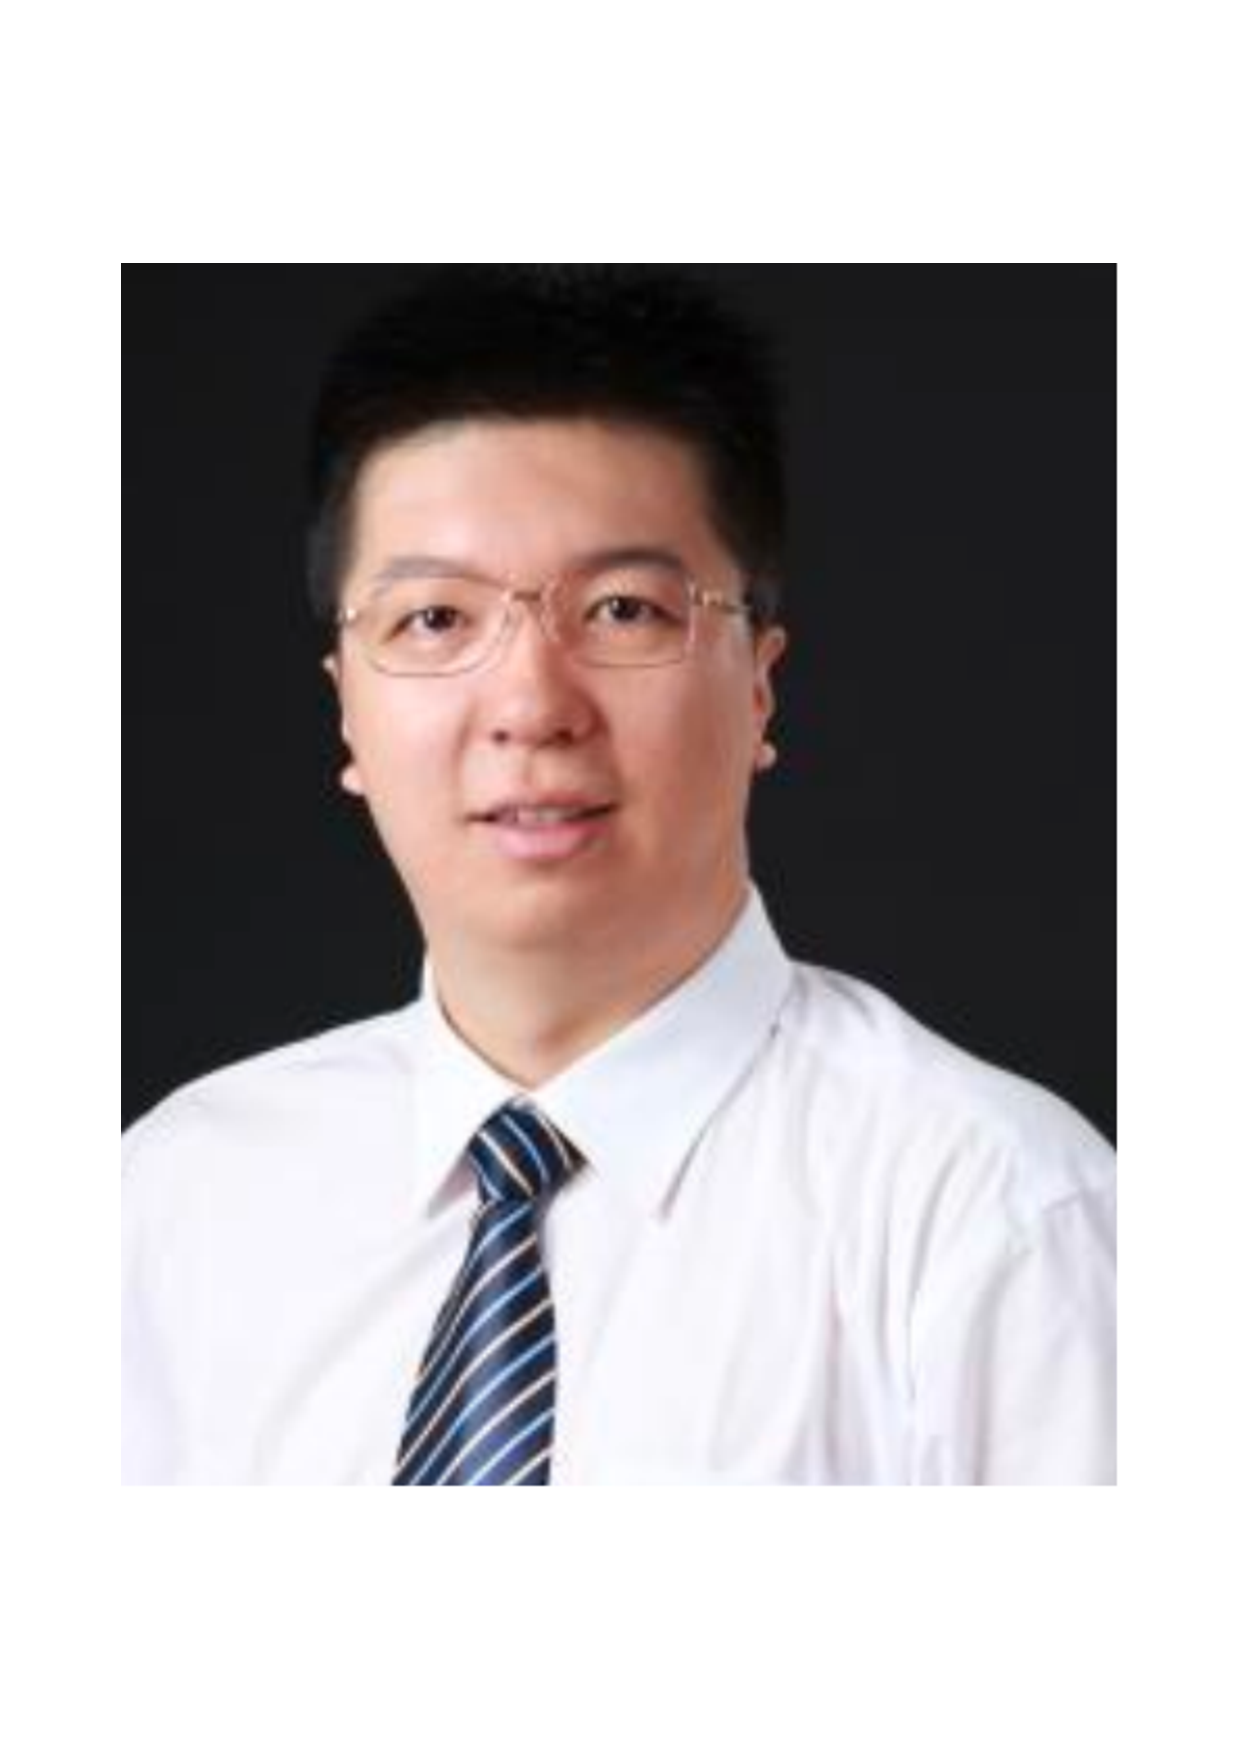
\includegraphics[width=1.5in,height=1.5in,clip,keepaspectratio]{bio/Figure_Zhang_Weizhe.pdf}}]{Weizhe Zhang} (Senior Member, IEEE) received the BEng, MEng, and PhD degrees of engineering in computer science and technology from the Harbin Institute of Technology in 1999, 2001, and 2006 respectively. He is currently a professor with the School of Computer Science and Technology, Harbin Institute of Technology, China, and the director of the Cyberspace Security Research Center, Peng Cheng Laboratory, Shenzhen, China. He has authored or coauthored more than 100 academic papers in journals, books, and conference proceedings. His research interests include parallel computing, distributed computing, cloud and grid computing, and computer network.
\end{IEEEbiography}
\vspace{-1.2cm}
\begin{IEEEbiography}[{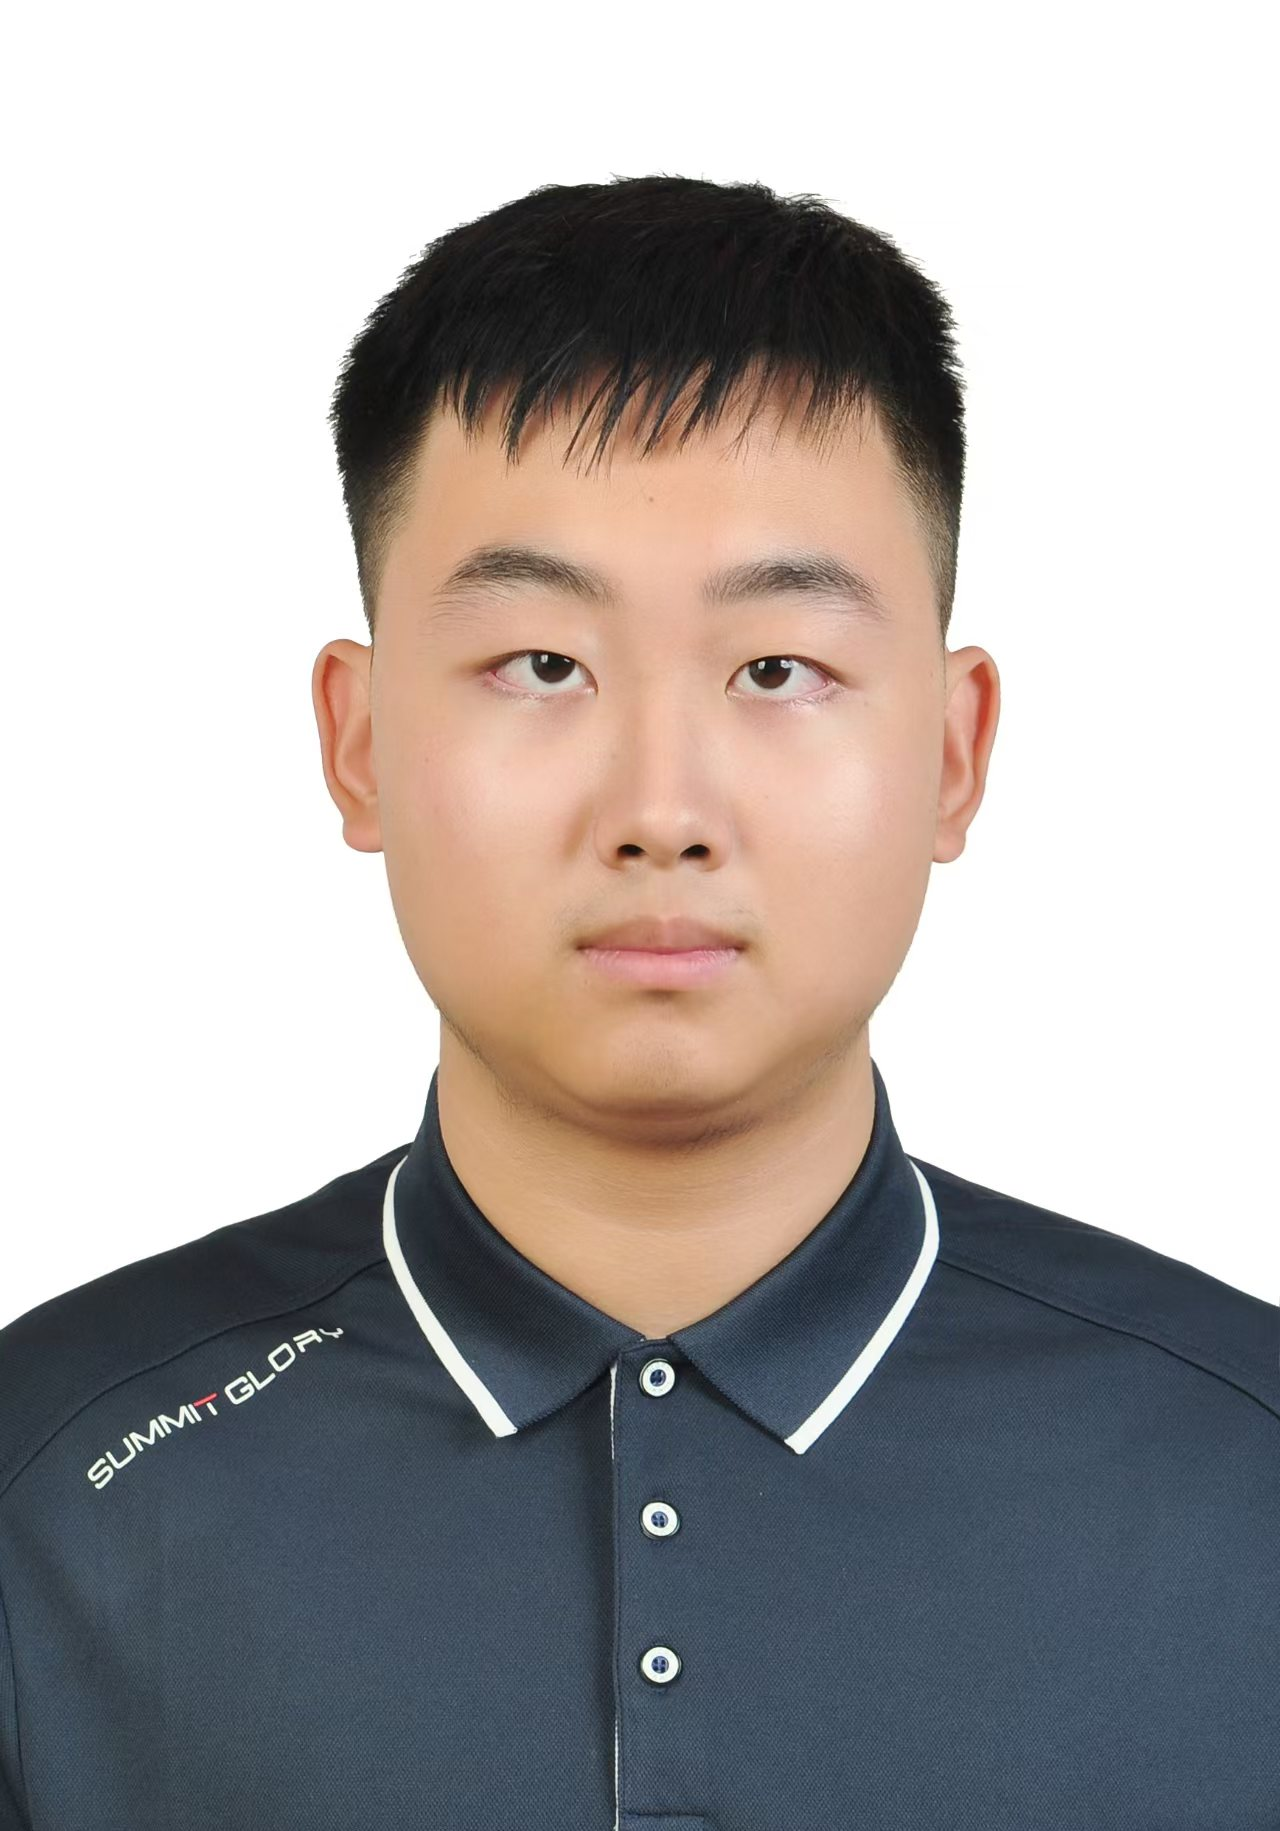
\includegraphics[width=0.8in,height=1.15in,clip,keepaspectratio]{bio/Figure_Li_Jiaxi.jpg}}]{Jiaxi Li} is currently an undergraduate student at the School of Computer Science and Technology, Harbin Institute of Technology, China, and is expected to pursue a Master's degree starting in September 2026. His research focuses on high-performance computing and artificial intelligence, with a particular focus on scheduling optimization for large language model inference systems.
\end{IEEEbiography}
\vspace{-1.2cm}
\begin{IEEEbiography}[{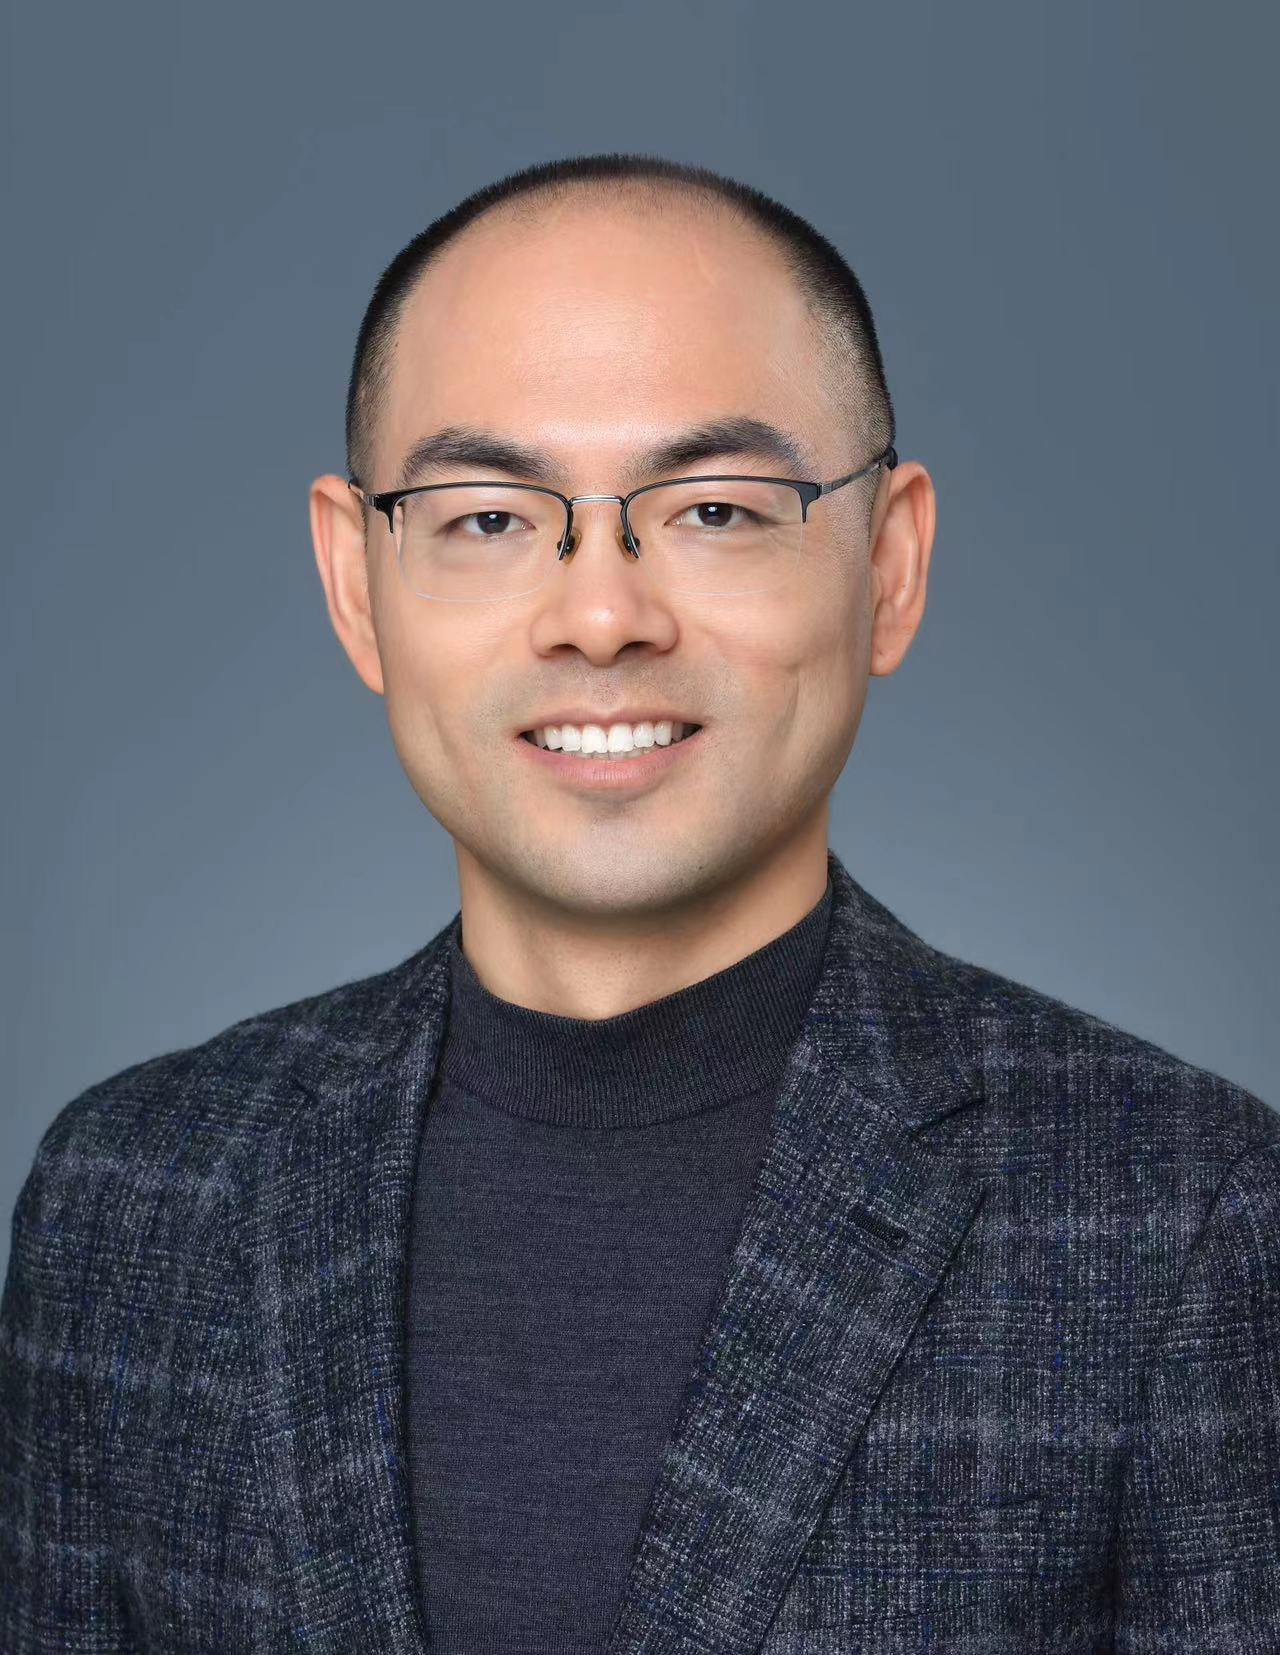
\includegraphics[width=0.8in,height=1.8in,clip,keepaspectratio]{bio/Figure_Hongwei_Yang.jpg}}]{Hongwei Yang} is a research associate of the Network Security Center in the School of Cyberspace Science, Harbin Institute of Technology, China. He received the DEng degree in cyberspace science from the Harbin Institute of Technology. His research interests include graph mining, privacy-preserving computing, network security, and big data security.
\end{IEEEbiography}
\vspace{-1.2cm}
\begin{IEEEbiography}[{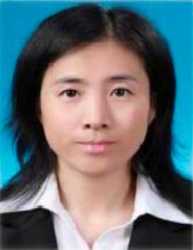
\includegraphics[width=0.8in,height=1.15in,clip,keepaspectratio]{bio/Figure_Hui_He.png}}]{Hui He} received the B.Eng, M.Eng, and Ph.D. degrees from the Harbin Institute of Technology, Harbin, China, in 1997, 1999, and 2006, respectively, all in computer science and technology. She is a Professor in the School of Cyberspace Science, Harbin Institute of Technology. Her current research interests include distributed computing, the Internet of Things, and big data analysis.
\end{IEEEbiography}
\vspace{-1.2cm}
\begin{IEEEbiography}[{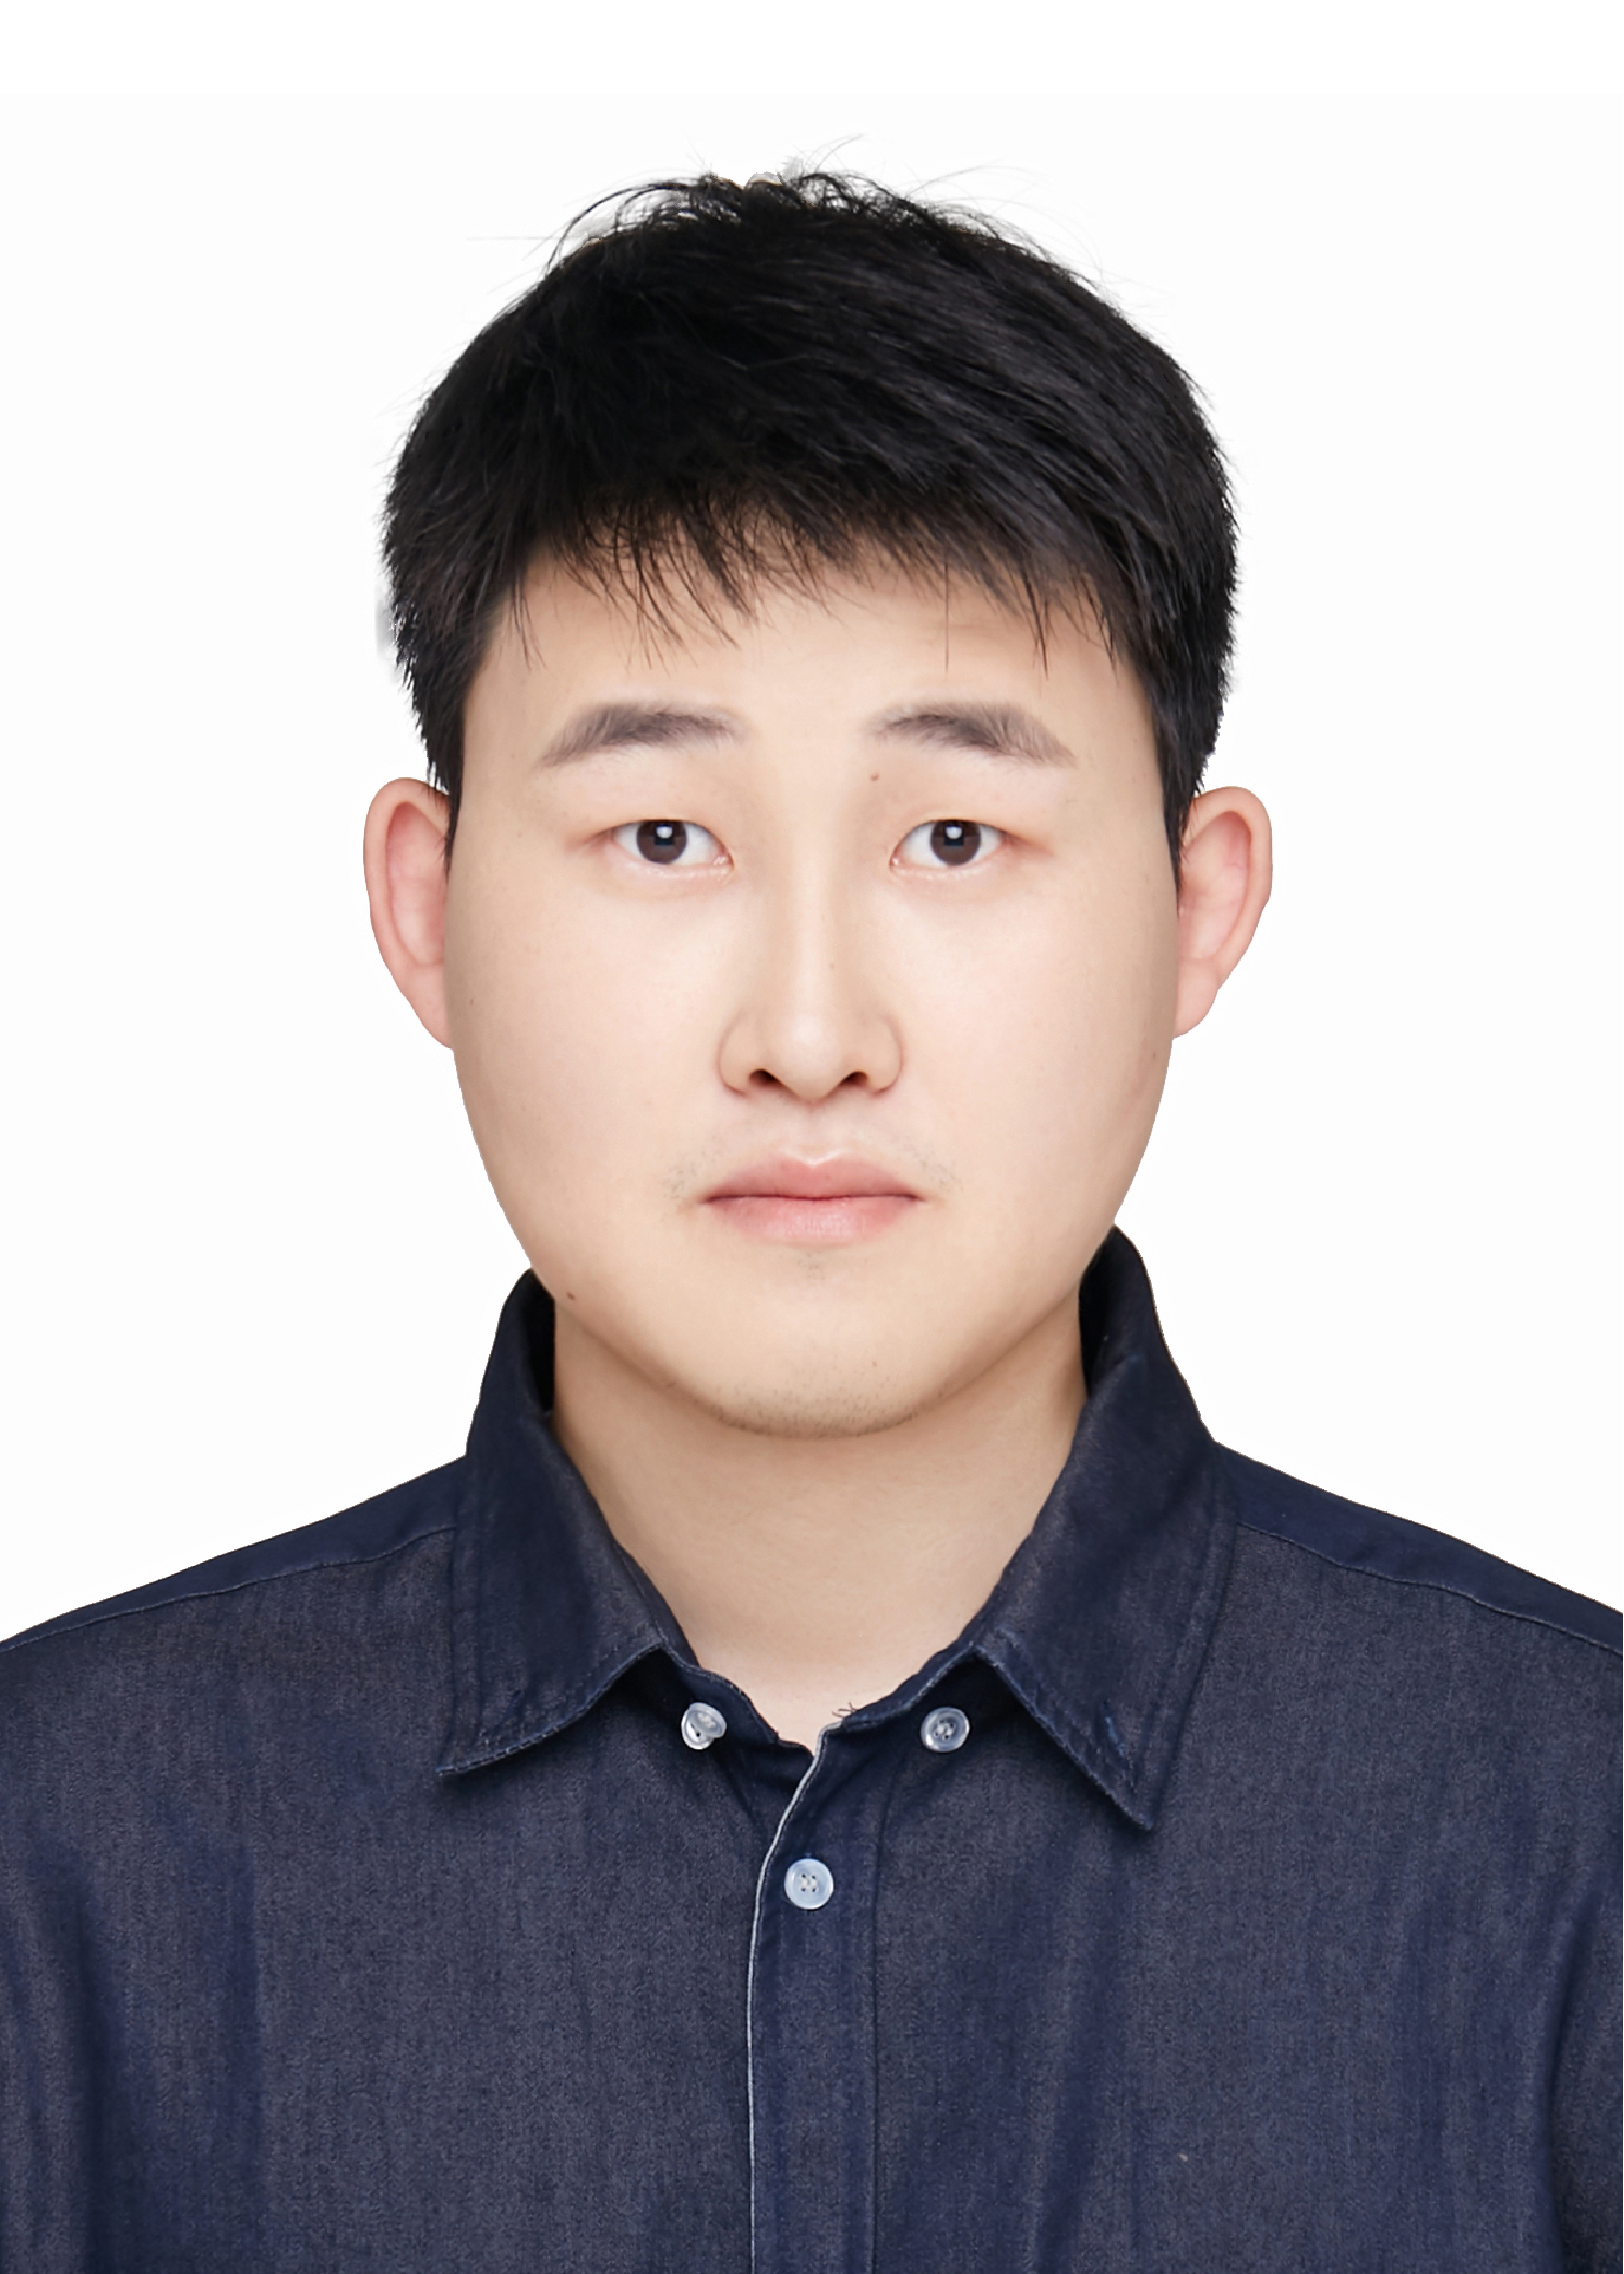
\includegraphics[width=0.8in,height=1.8in,clip,keepaspectratio]{bio/Figure_DESHENG_WANG.pdf}}]{Desheng Wang} received the Ph.D. degree in Cyberspace Security from Harbin Institute of Technology, Harbin, China, in 2022. He is currently an assistant professor in the School of Computer Science and Technology at Harbin Institute of Technology, Shenzhen, China. His research interests include cloud computing, edge computing, and cyberspace security. 
\end{IEEEbiography}
\end{document}
